
\documentclass[11pt, class=report,crop=false]{standalone}
\usepackage[screen]{../exo7book}


\begin{document}

% Constantes pour l'inclusion des figures
\newcommand{\myscale}{1}


%====================================================================
\chapitre{Fonctions de plusieurs variables}
%====================================================================



%%%%%%%%%%%%%%%%%%%%%%%%%%%%%%%%%%%%%%%%%%%%%%%%%%%%%
\section{Introduction}

En première année, vous avez étudié les fonctions d'une variable : par exemple, si $t\mapsto f(t)$ représente l'évolution d'une population en fonction du temps, vous savez déterminer ses caractéristiques (croissance, maximum, limite...). 
Mais de nombreux phénomènes dépendent de plusieurs paramètres : par exemple, le volume d'un gaz dépend de la température et de la pression, ou bien l'altitude  d'un point à la surface de la Terre dépend de la latitude et de la longitude. Le but de ce cours est de faire le même travail que pour les fonctions d'une variable : étudier la croissance, les maximums, les limites... Bien sûr, la situation est plus délicate, mais aussi plus intéressante, du fait qu'il y a plusieurs variables !

\begin{center}
    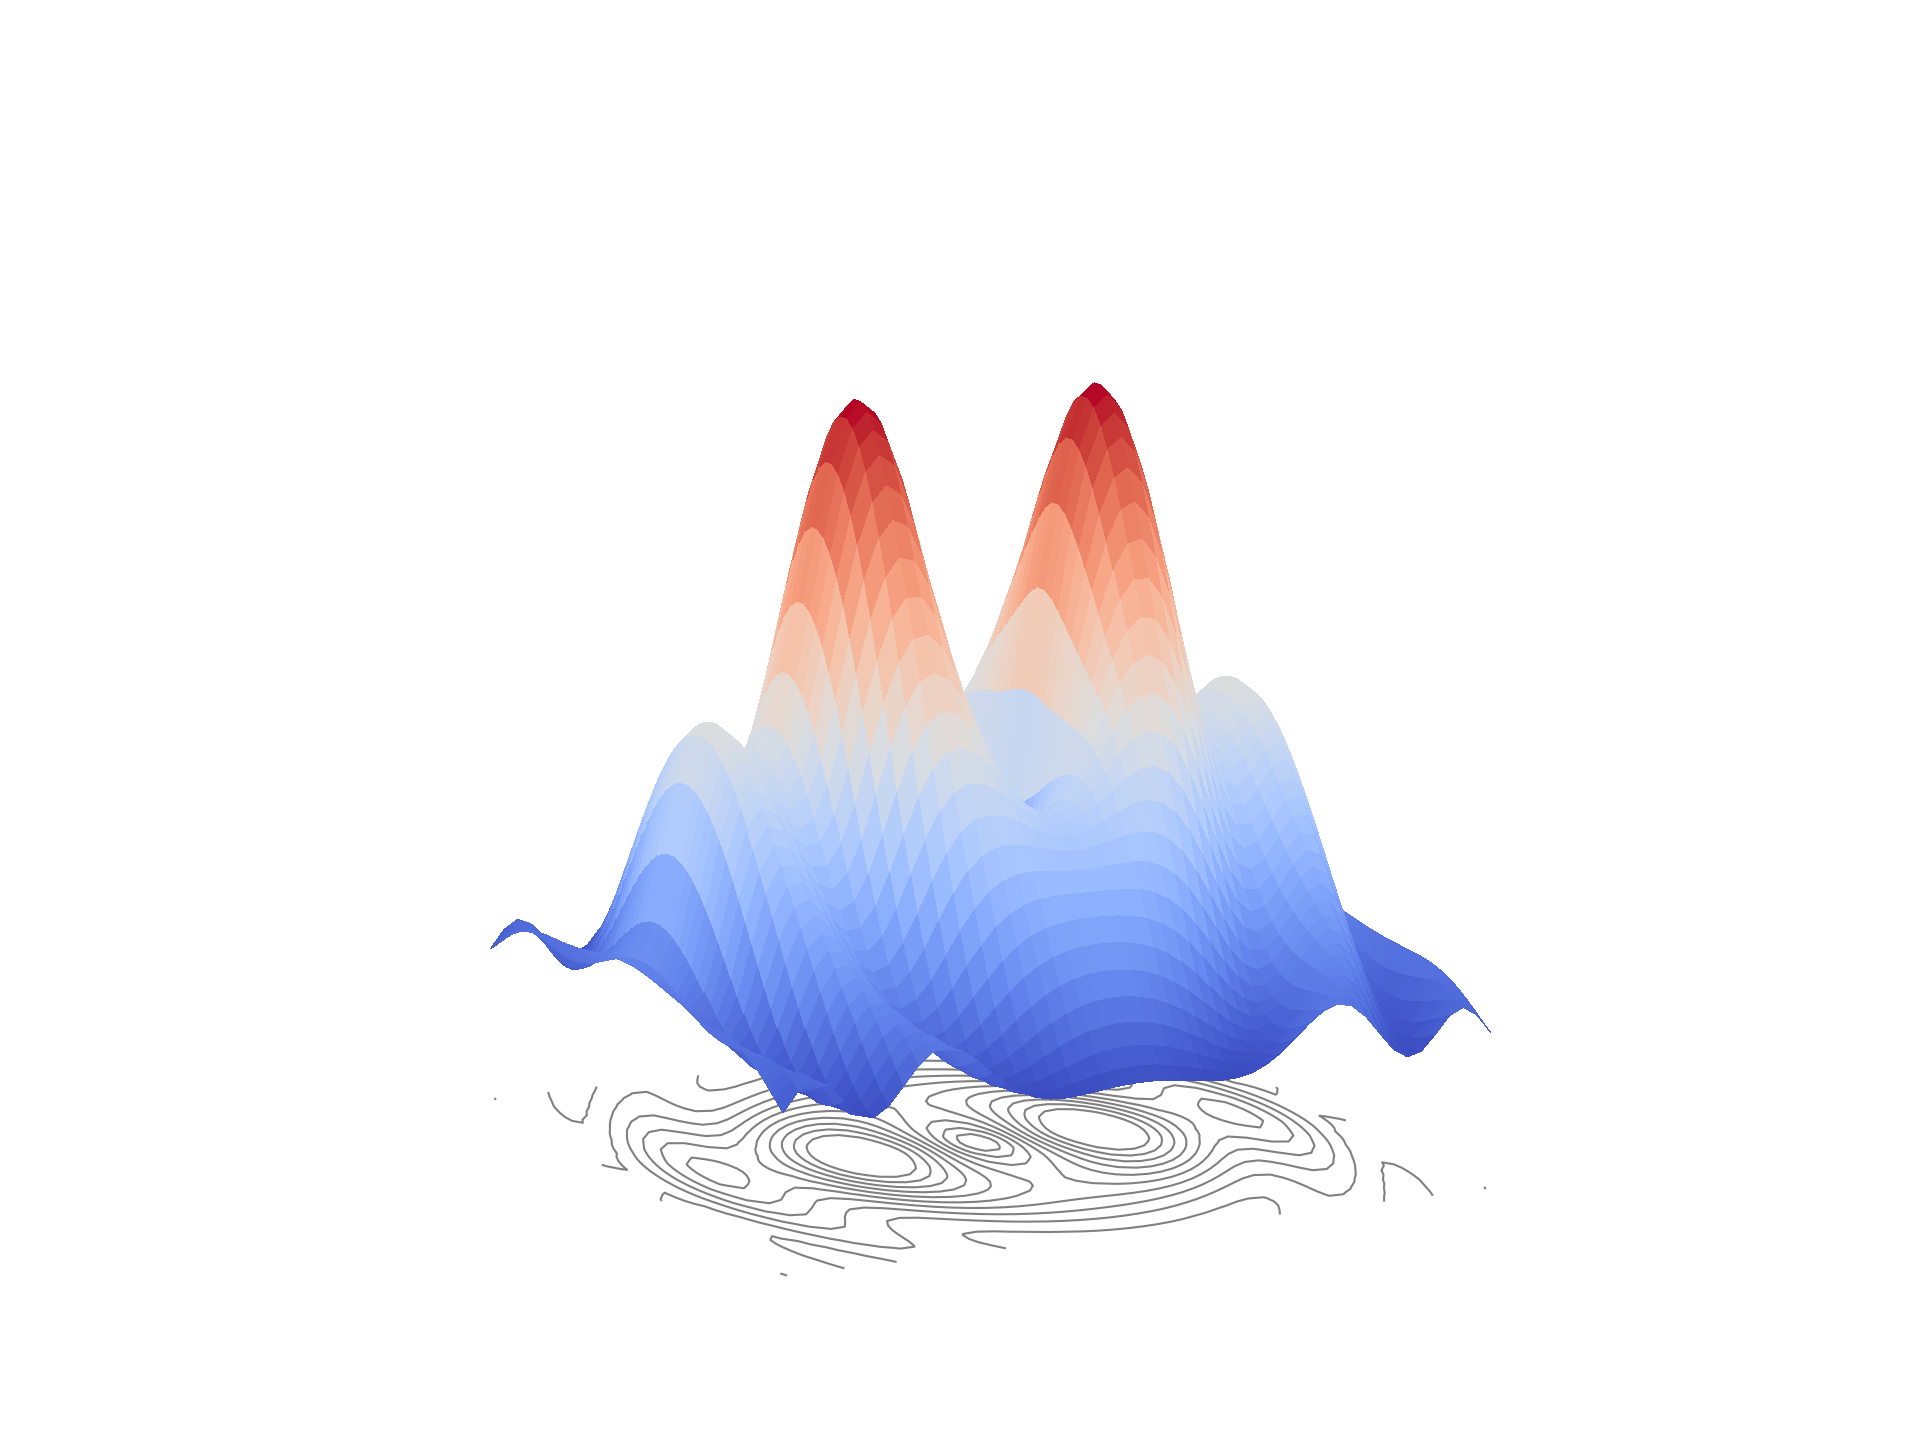
\includegraphics[trim={4cm 1cm 3cm 3cm}, clip, scale=\myscale, scale=0.8]{figures/fonctions-niveau-3a}
\end{center}

%----------------------------------------------------
\subsection{Que sont les fonctions de plusieurs variables ?}

Dans ce chapitre, nous allons étudier les fonctions de plusieurs variables dans le cadre particulier de $\Rr^2$ ou $\Rr^3$, mais également dans le cadre général de $\Rr^n$. Ces fonctions seront donc de la forme 
\begin{equation*}
f:E \subset \Rr^n \rightarrow \Rr,
\end{equation*}
où $n\ge 1$ est un entier naturel. 

Autrement dit, les éléments de l'ensemble de départ $E$ seront des $n$-uplets du type $(x_1,\ldots,x_n)$ que l'on peut considérer comme des vecteurs, et les éléments de l'ensemble d'arrivée seront des réels.


\begin{exemple}
\sauteligne
\begin{enumerate}
\item $n=1$. $f: I \subset \R \rightarrow \R$:  c'est le cas le plus simple,
$x \mapsto f(x)$, celui qui est connu depuis le lycée. Voici les graphes des fonctions $x \mapsto x \cdot \cos(x)$ et $x \mapsto \arccos(x)$ :

\myfigure{1.2}{
  \tikzinput{fig-plusvar-11-01}\qquad
  \tikzinput{fig-plusvar-11-02}
} 

\item $n=2$. $f: E \subset \Rr^2 \rightarrow \Rr$. 
On préfère noter les variables par $(x,y)$ (au lieu de $(x_1,x_2)$).
Ces fonctions $(x,y) \mapsto f(x,y)$ seront notre principal sujet d'étude et sont représentées par des surfaces. 
À gauche, le graphe de la fonction $ (x,y) \mapsto \sin(y)e^{-x^2}$.
À droite, le graphe de la fonction $ (x,y) \mapsto \sin(xy)$.
\begin{center}
    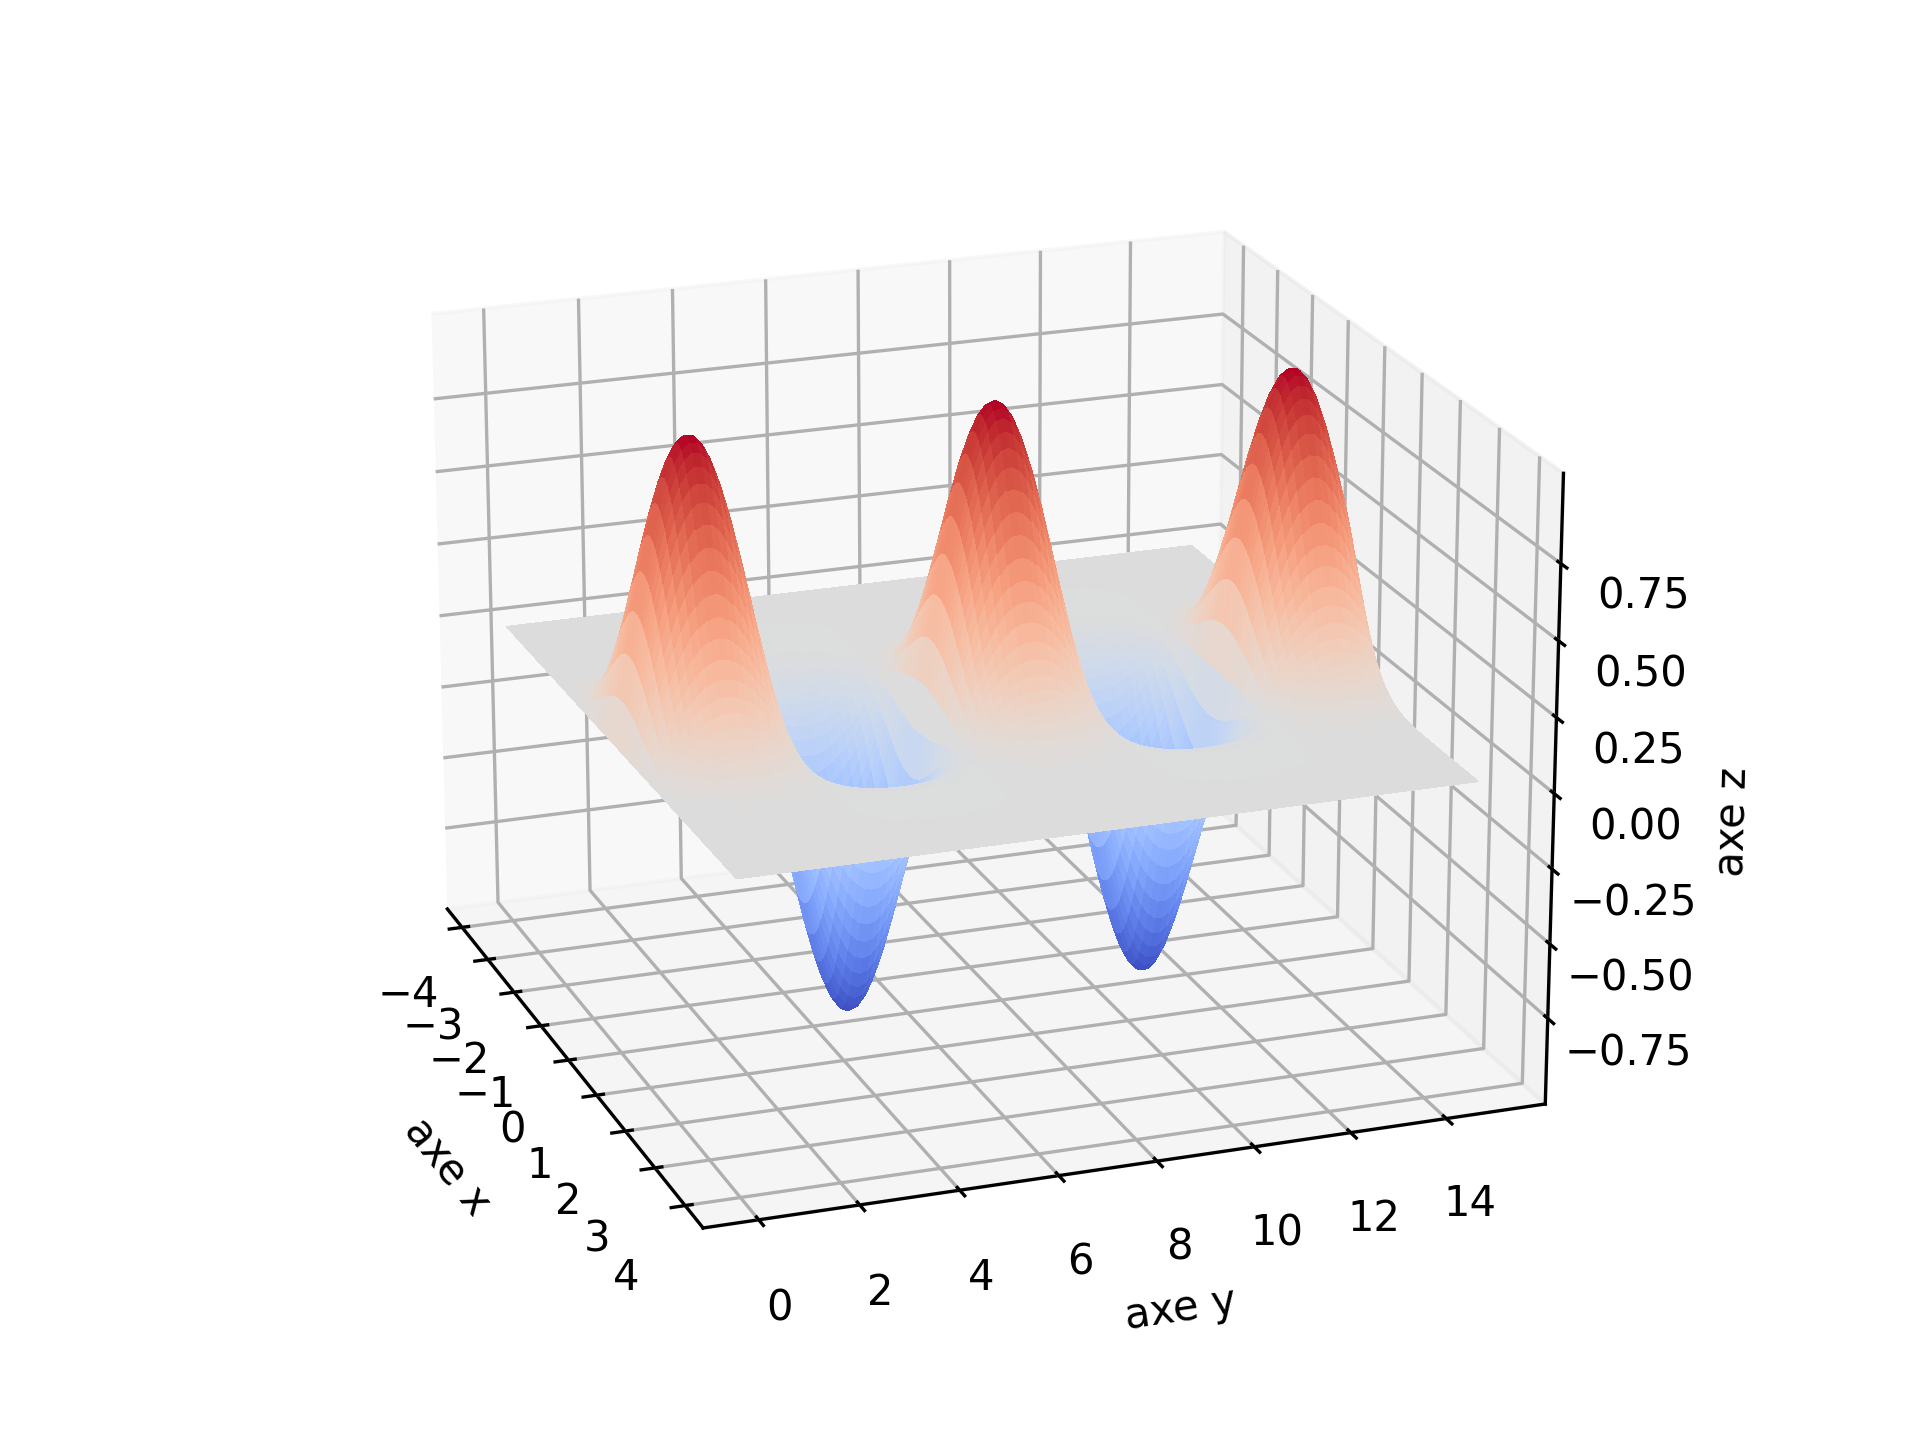
\includegraphics[scale=\myscale,scale=0.5]{figures/fonctions-intro-01}
    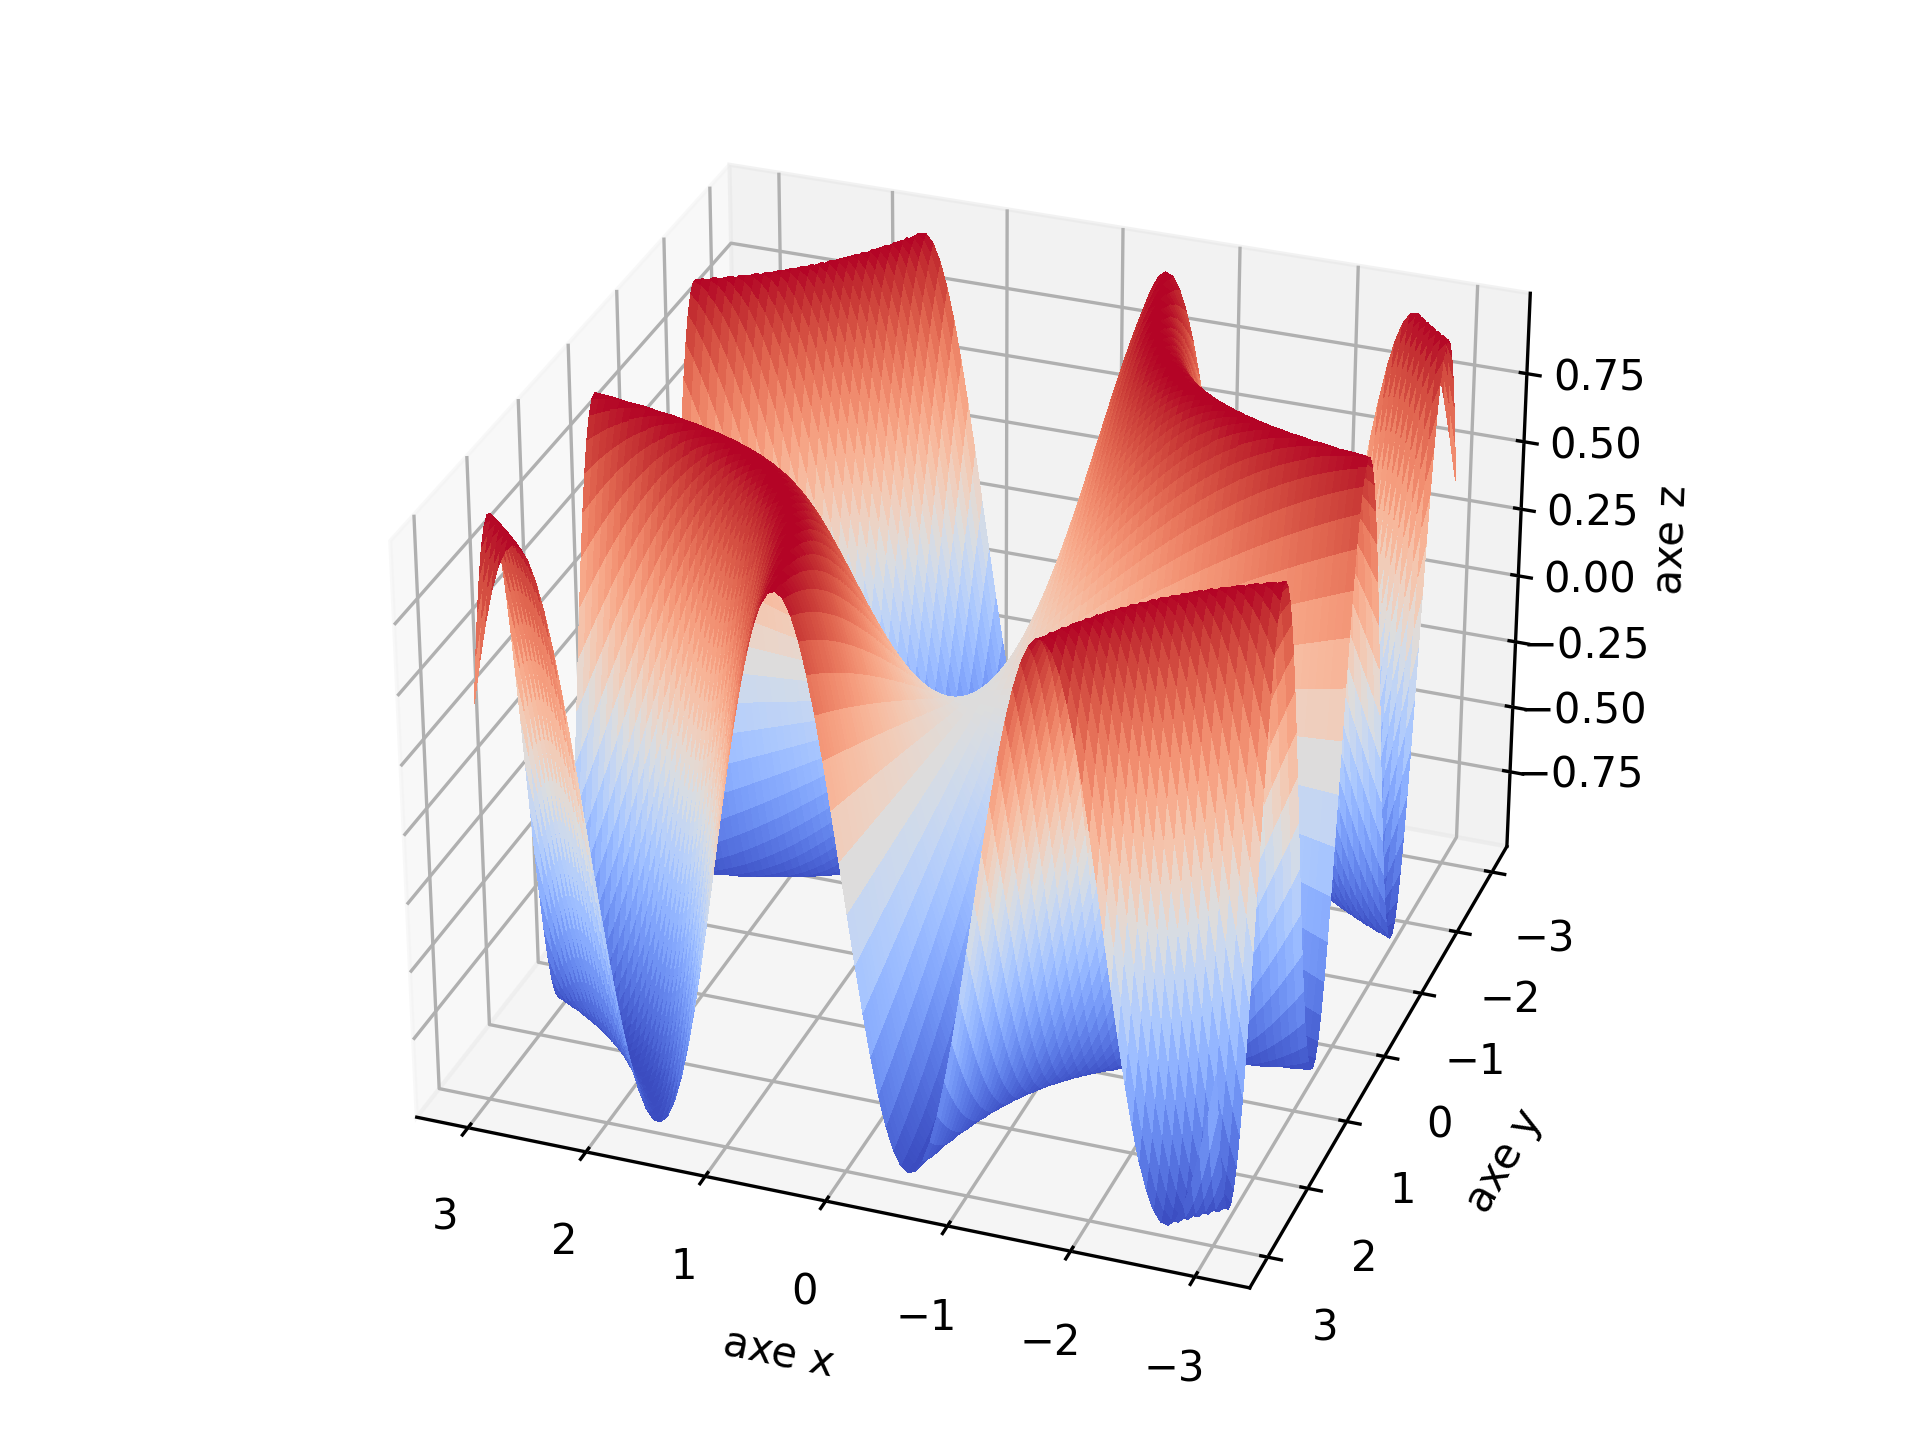
\includegraphics[scale=\myscale,scale=0.5]{figures/fonctions-intro-02}
\end{center}

% dessins 3d voir 'fonctions-intro-01.py' et 'fonctions-intro-02.py' 
\end{enumerate}
\end{exemple}

Dès que $n>2$, il est assez difficile d'avoir une vision graphique. 
  
\bigskip

Nous allons aussi étudier des fonctions, dites fonctions vectorielles, dont l'ensemble d'arrivée n'est pas $\Rr$, mais $\Rr^p$, donc de la forme 
\begin{equation*}
f:E \subset \Rr^n \rightarrow \Rr^p,
\end{equation*}
où $n\ge 1$ et $p\ge 1$ sont des entiers naturels. 

Dans ce cas, si $x=(x_1,\ldots,x_n)$ est un vecteur de $\Rr^n$, alors $f(x)$ est un vecteur de $\Rr^p$, du type $f(x)=(f_1(x_1,\ldots,x_n), \ldots,f_p(x_1,\ldots,x_n))$. Attention, dans la suite, $x$ désignera parfois le vecteur $x=(x_1,\ldots,x_n)$ et parfois $x$ désignera un seul réel (comme par exemple pour une fonction de deux variables $f(x,y)$).

\begin{exemple}
\sauteligne
\begin{enumerate}
 
\item $n=1$, $p=2$. $f: I \subset \Rr \rightarrow \Rr^2$ 
est représentée par une courbe paramétrée du plan.

Exemple : la fonction $f : \Rr \to \Rr^2$ définie par $t \mapsto (\sin(2t),\sin(3t))$.
Cela correspond à la courbe paramétrée définie par $x(t) = \sin(2t)$ et $y(t) = \sin(3t)$.
 
\begin{center}
    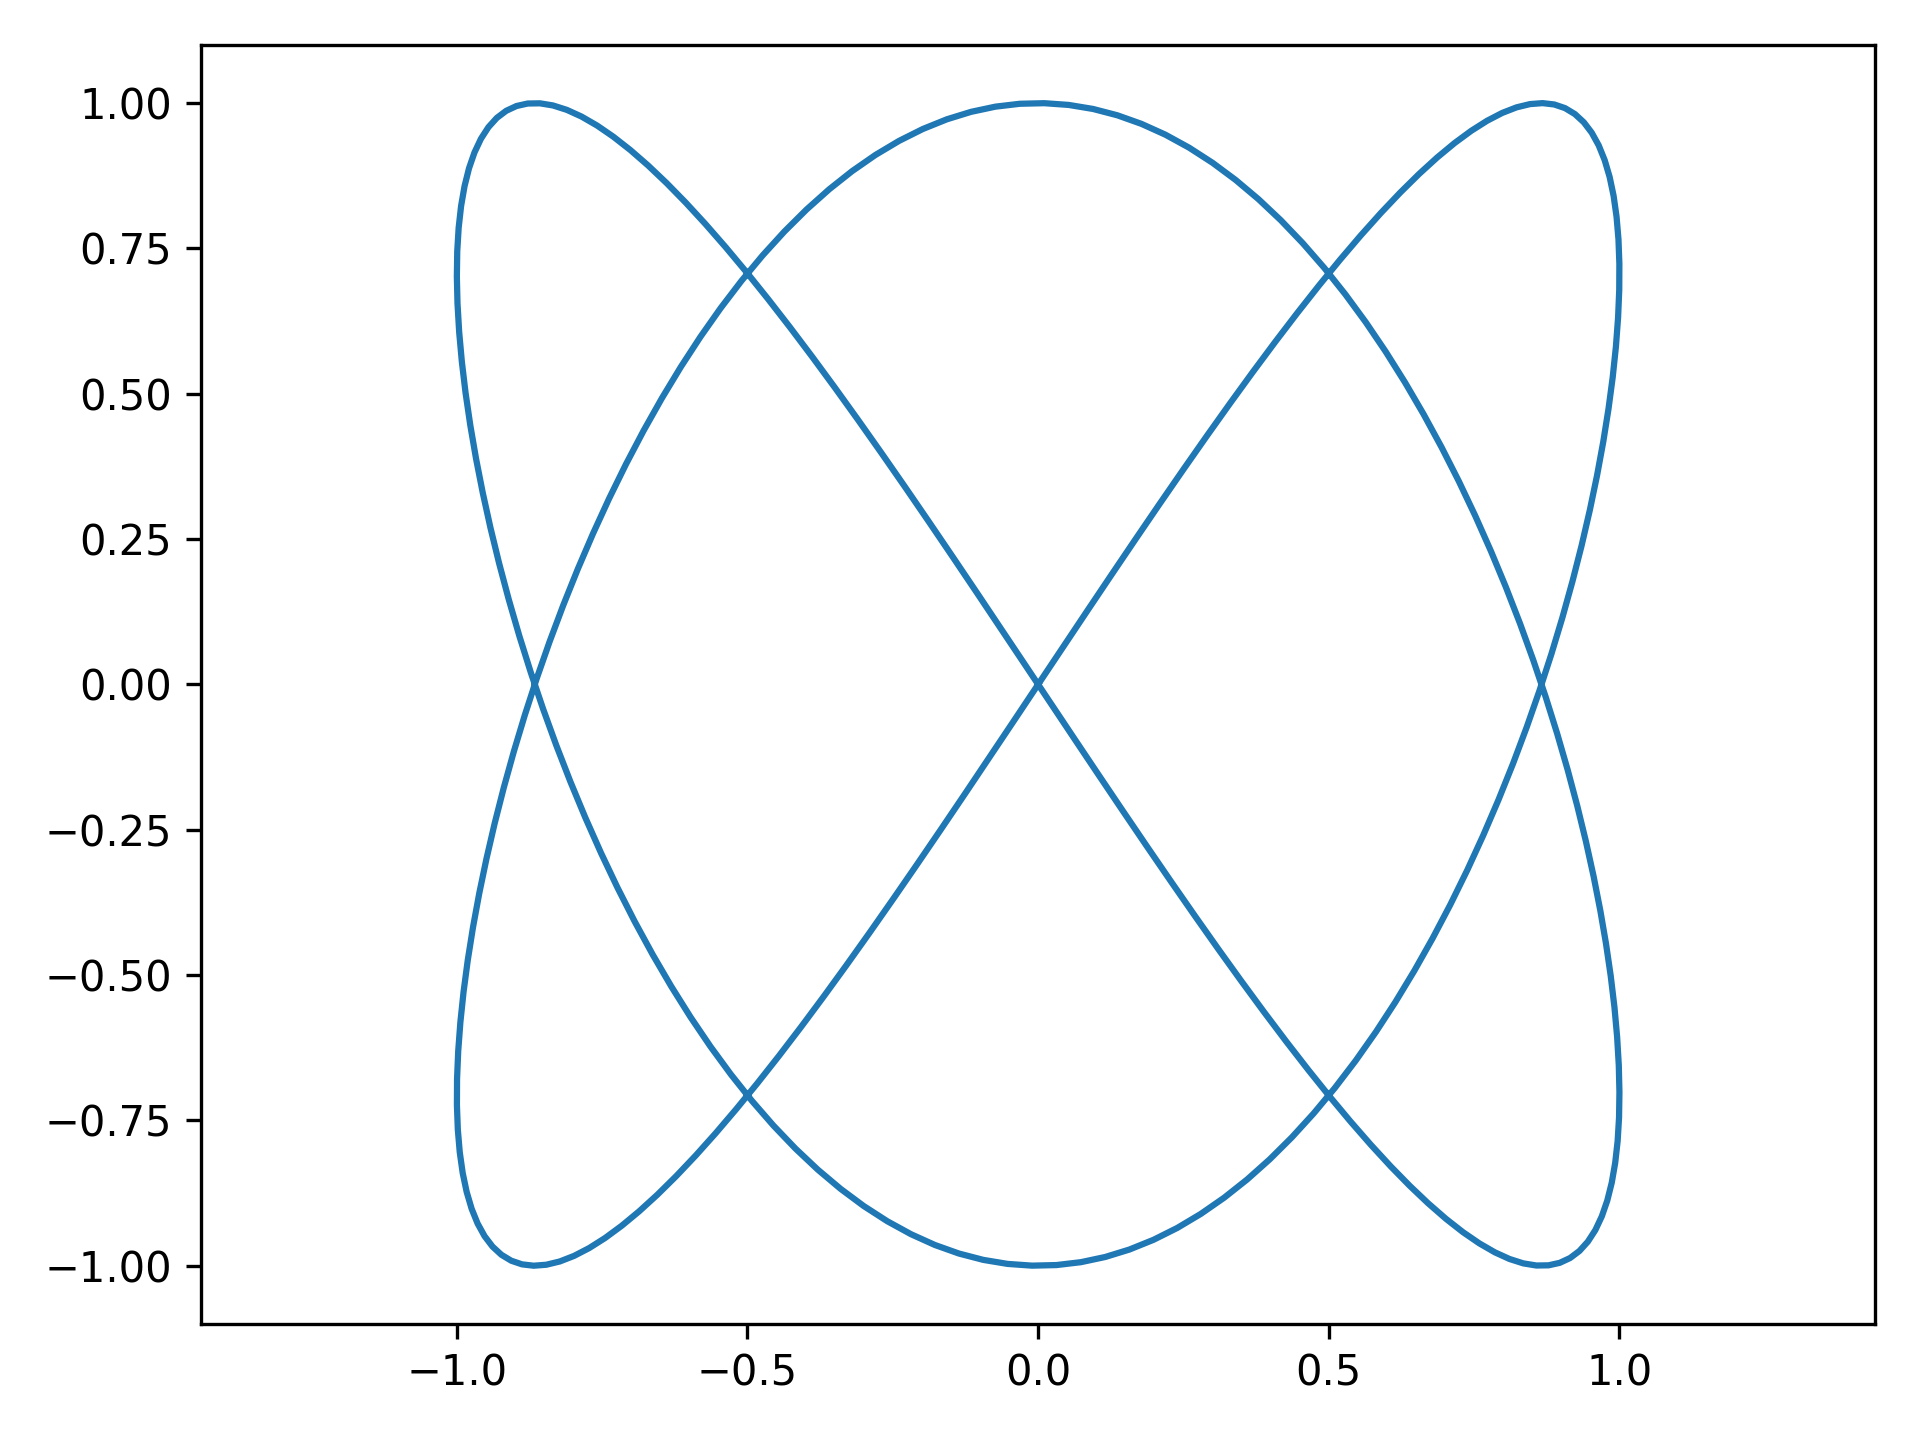
\includegraphics[scale=\myscale,scale=0.5]{figures/fonctions-intro-03}
\end{center}

% dessins 3d voir 'fonctions-intro-03.py' 

On peut interpréter le dessin comme l'ensemble des positions $(x(t),y(t)) \in \Rr^2$ que prend une particule dans le plan en fonction du temps $t \in \Rr$. 

\item $n=1$, $p=3$. $f: I \subset \Rr \rightarrow \Rr^3$ 
est représentée par une courbe paramétrée de l'espace.
Exemple : la fonction $f : \Rr \to \Rr^3$ définie par $t \mapsto (\cos t,\sin t, t)$.
Cela correspond au mouvement dans l'espace d'une particule $(x(t),y(t),z(t))$, qui ici parcourt une hélice.
\begin{center}
    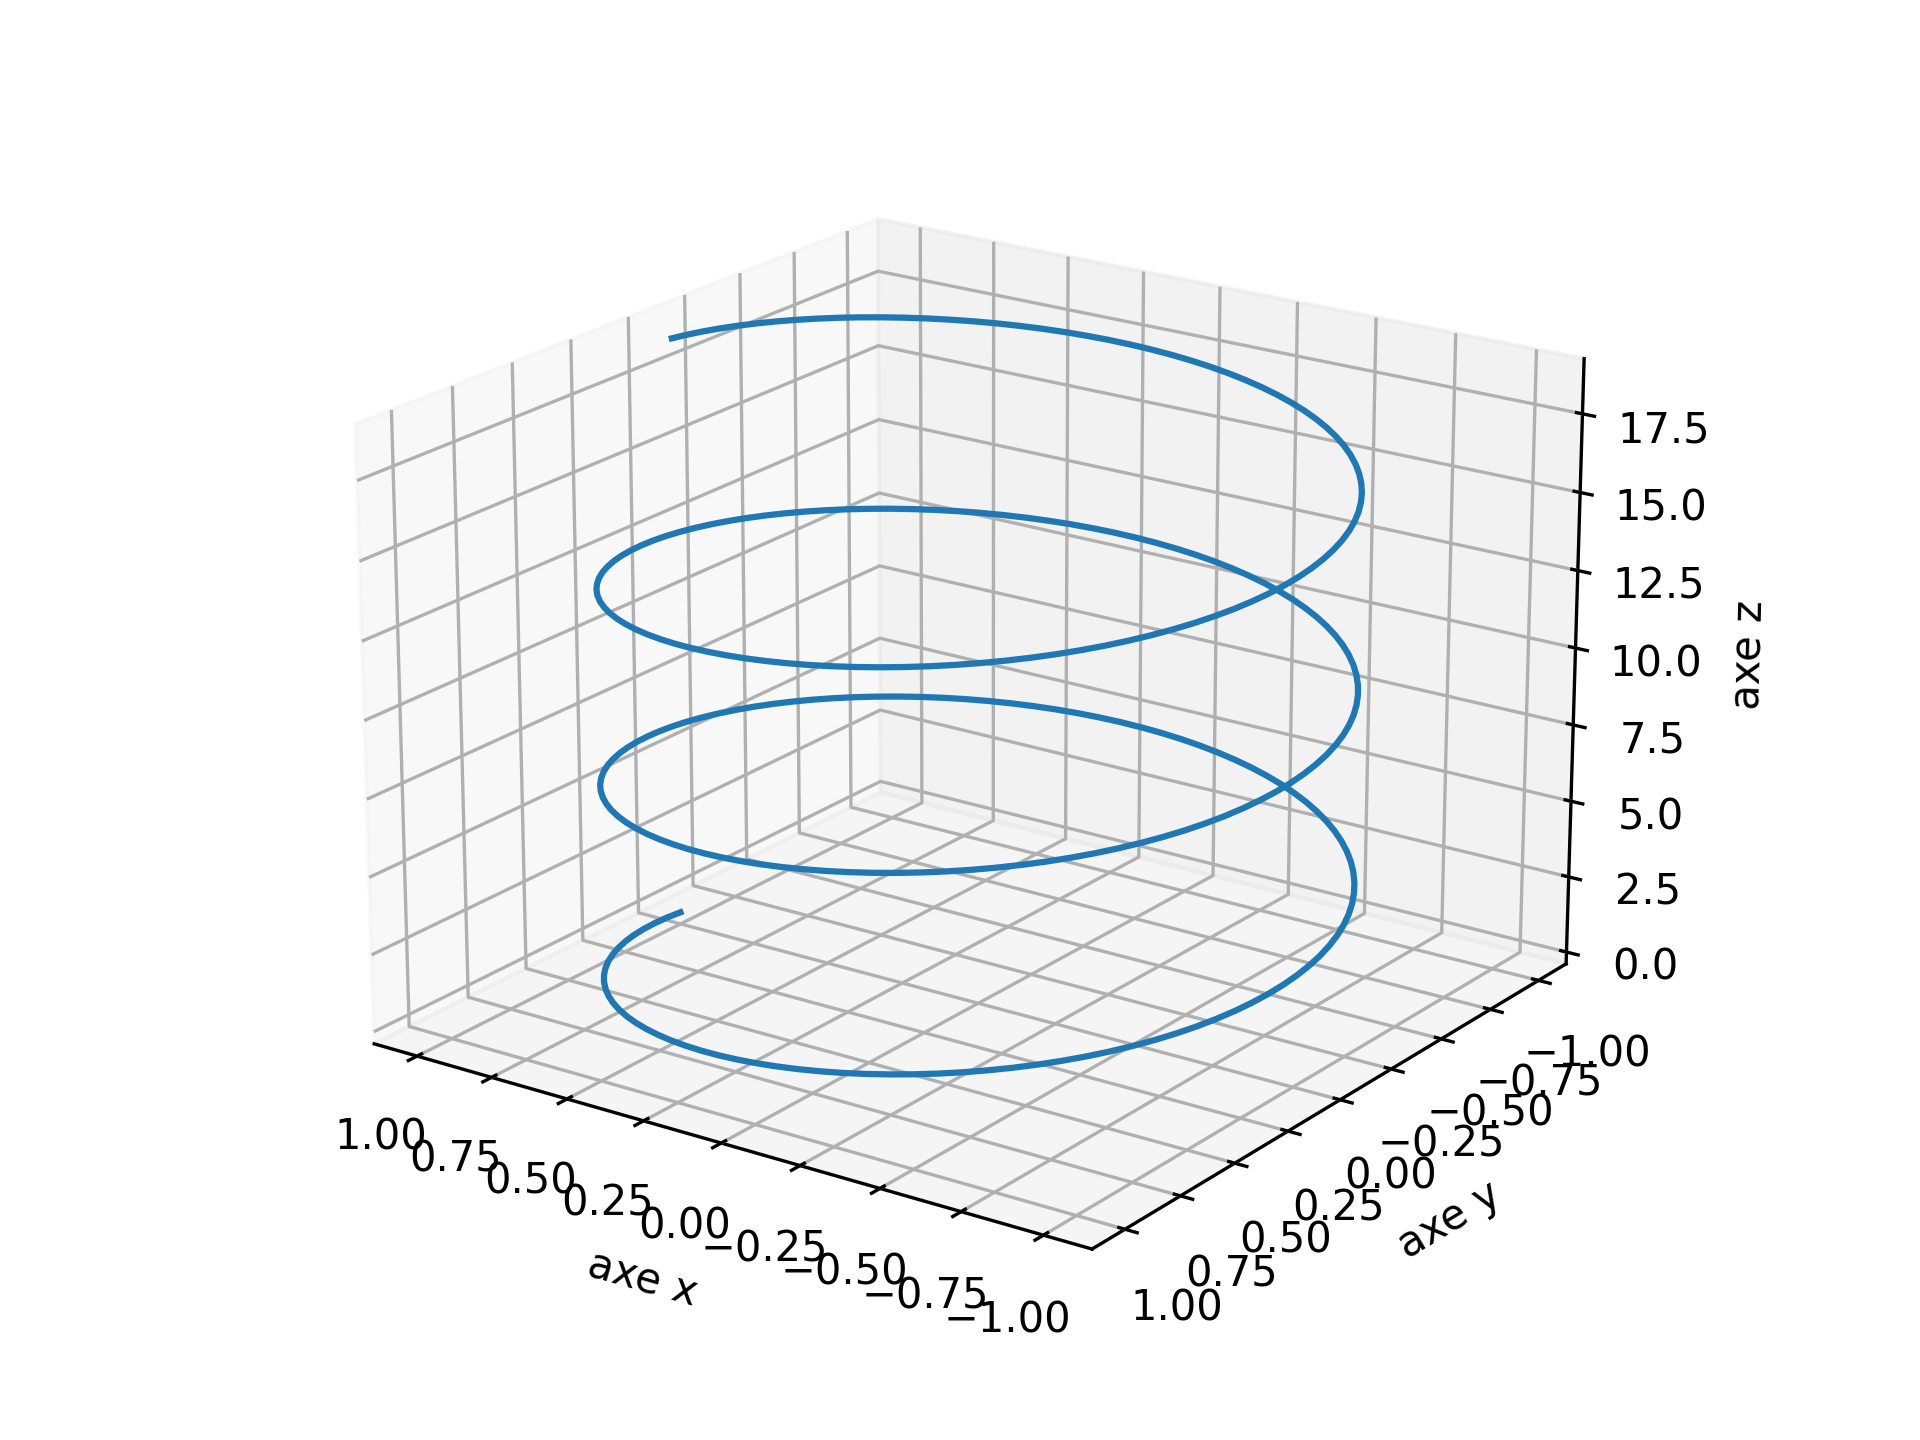
\includegraphics[scale=\myscale,scale=0.5]{figures/fonctions-intro-04}
\end{center}

% dessins 3d voir 'fonctions-intro-04.py'  

       
\item $n=2$, $p=3$. $f: E \subset \Rr^2 \rightarrow \Rr^3$: elles sont représentées par exemple par des surfaces paramétrées.

Voici l'exemple de la fonction 
$$(u,v) \mapsto \big( (2+\sin v)\cos u, (2+\sin v)\sin u,u+\cos v \big).$$
Chaque paramètre $(u,v) \in \Rr^2$ correspond à un point $(x(u,v),y(u,v),z(u,v)) \in \Rr^3$ de la surface hélicoïdale.

\begin{center}
    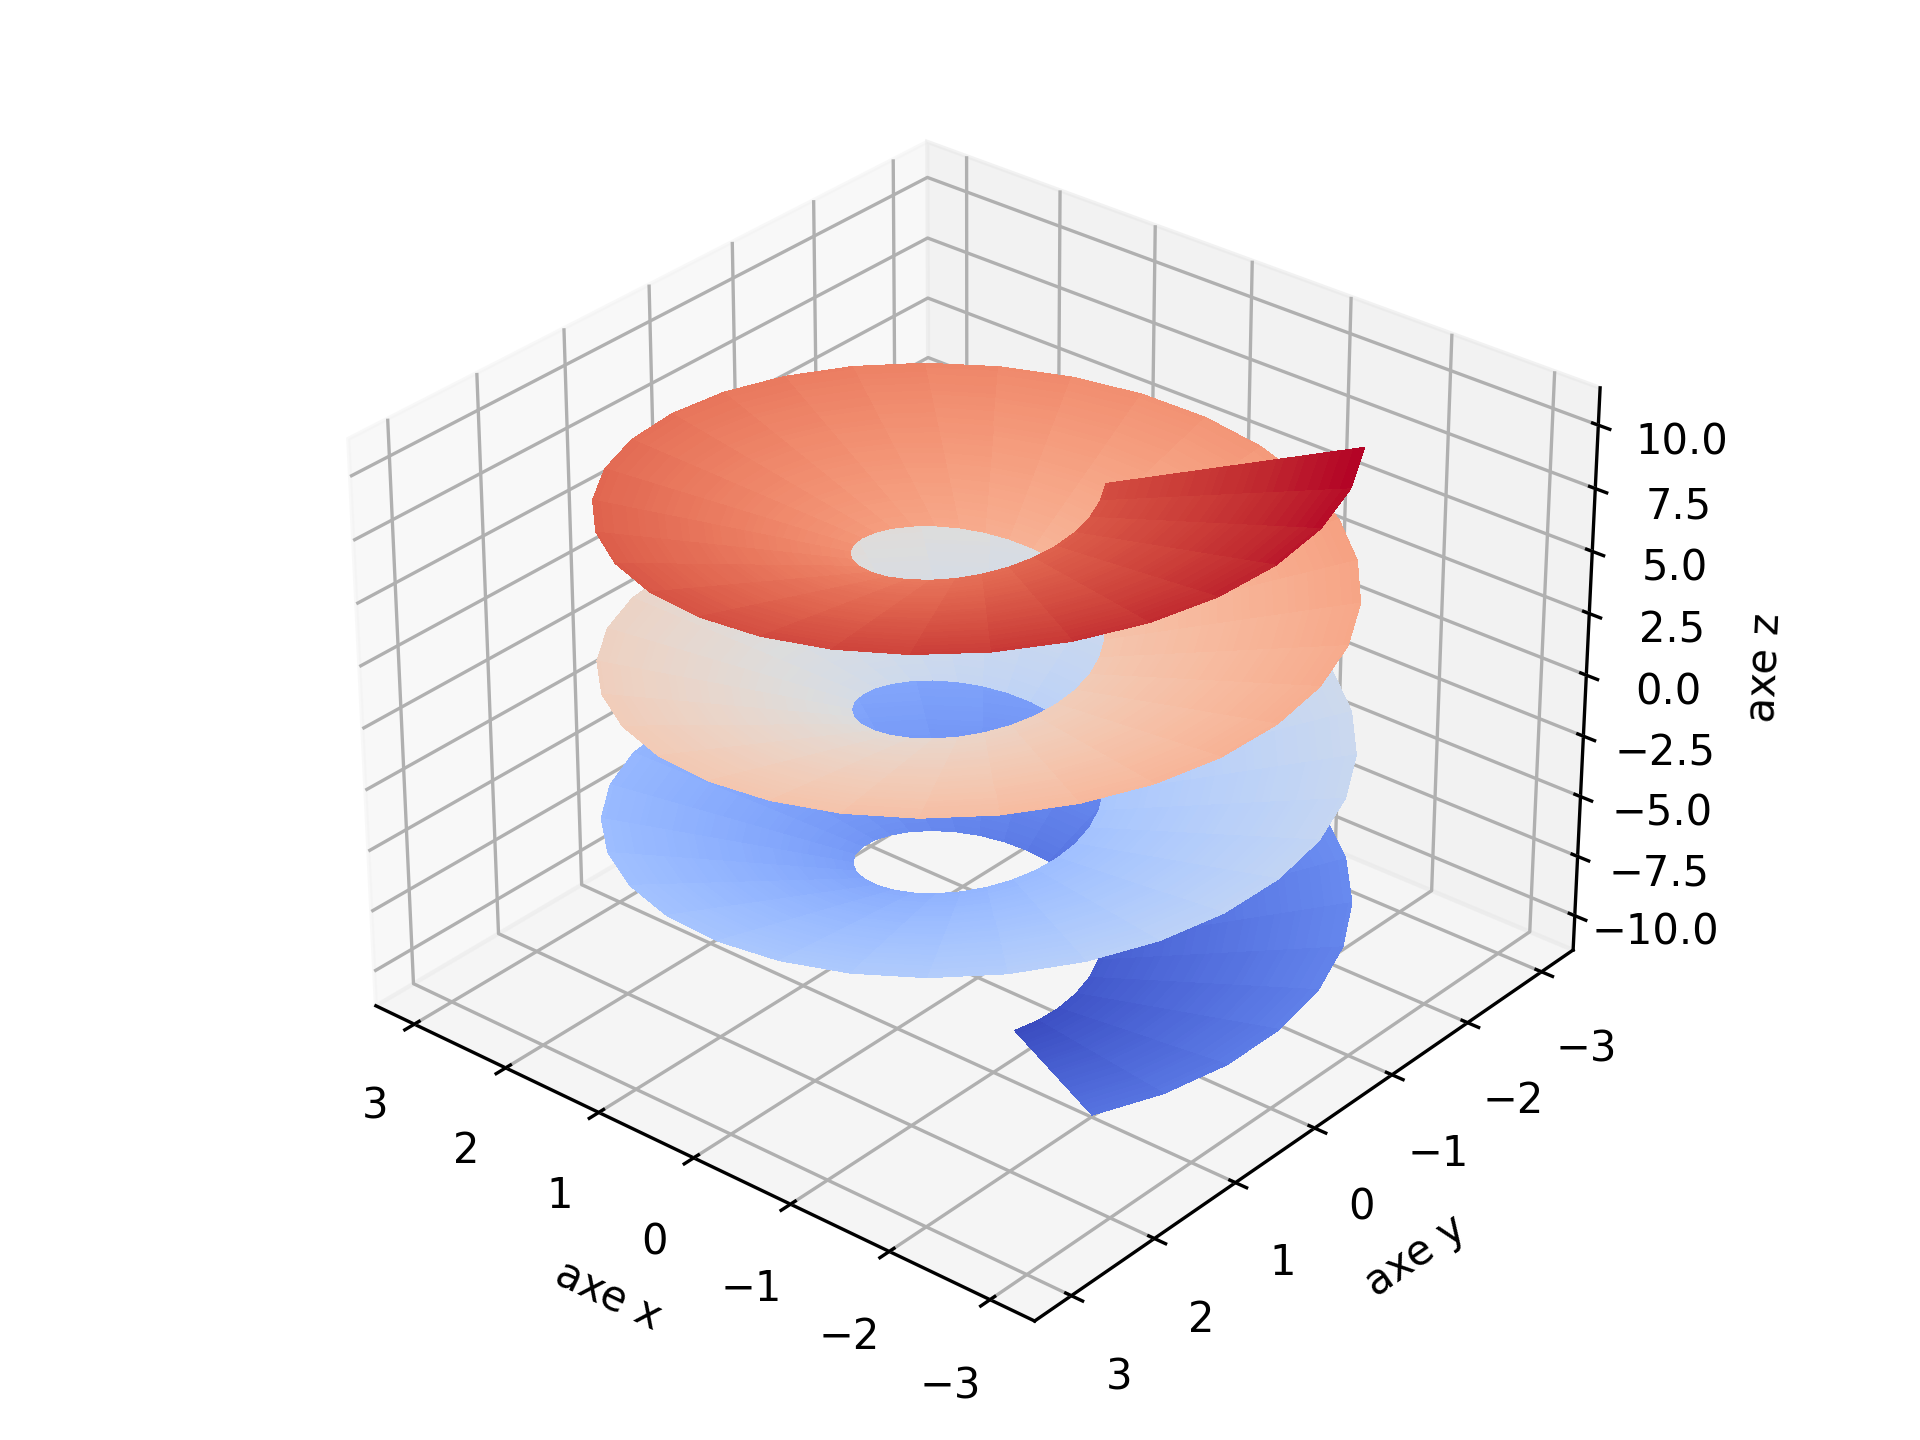
\includegraphics[scale=\myscale,scale=0.6]{figures/fonctions-intro-05}
\end{center}

% dessins 3d voir 'fonctions-intro-05.py'
 

\item $n=2$, $p = 2$. $f: E \subset \Rr^2 \rightarrow \Rr^2$: elles sont représentées par exemple par des champs de vecteurs.
À chaque point du plan $(x,y)$ on associe le vecteur $\vec v = f(x,y)$. (Sur la figure ci-dessous, seuls certains vecteurs sont représentés.)

\begin{center}
    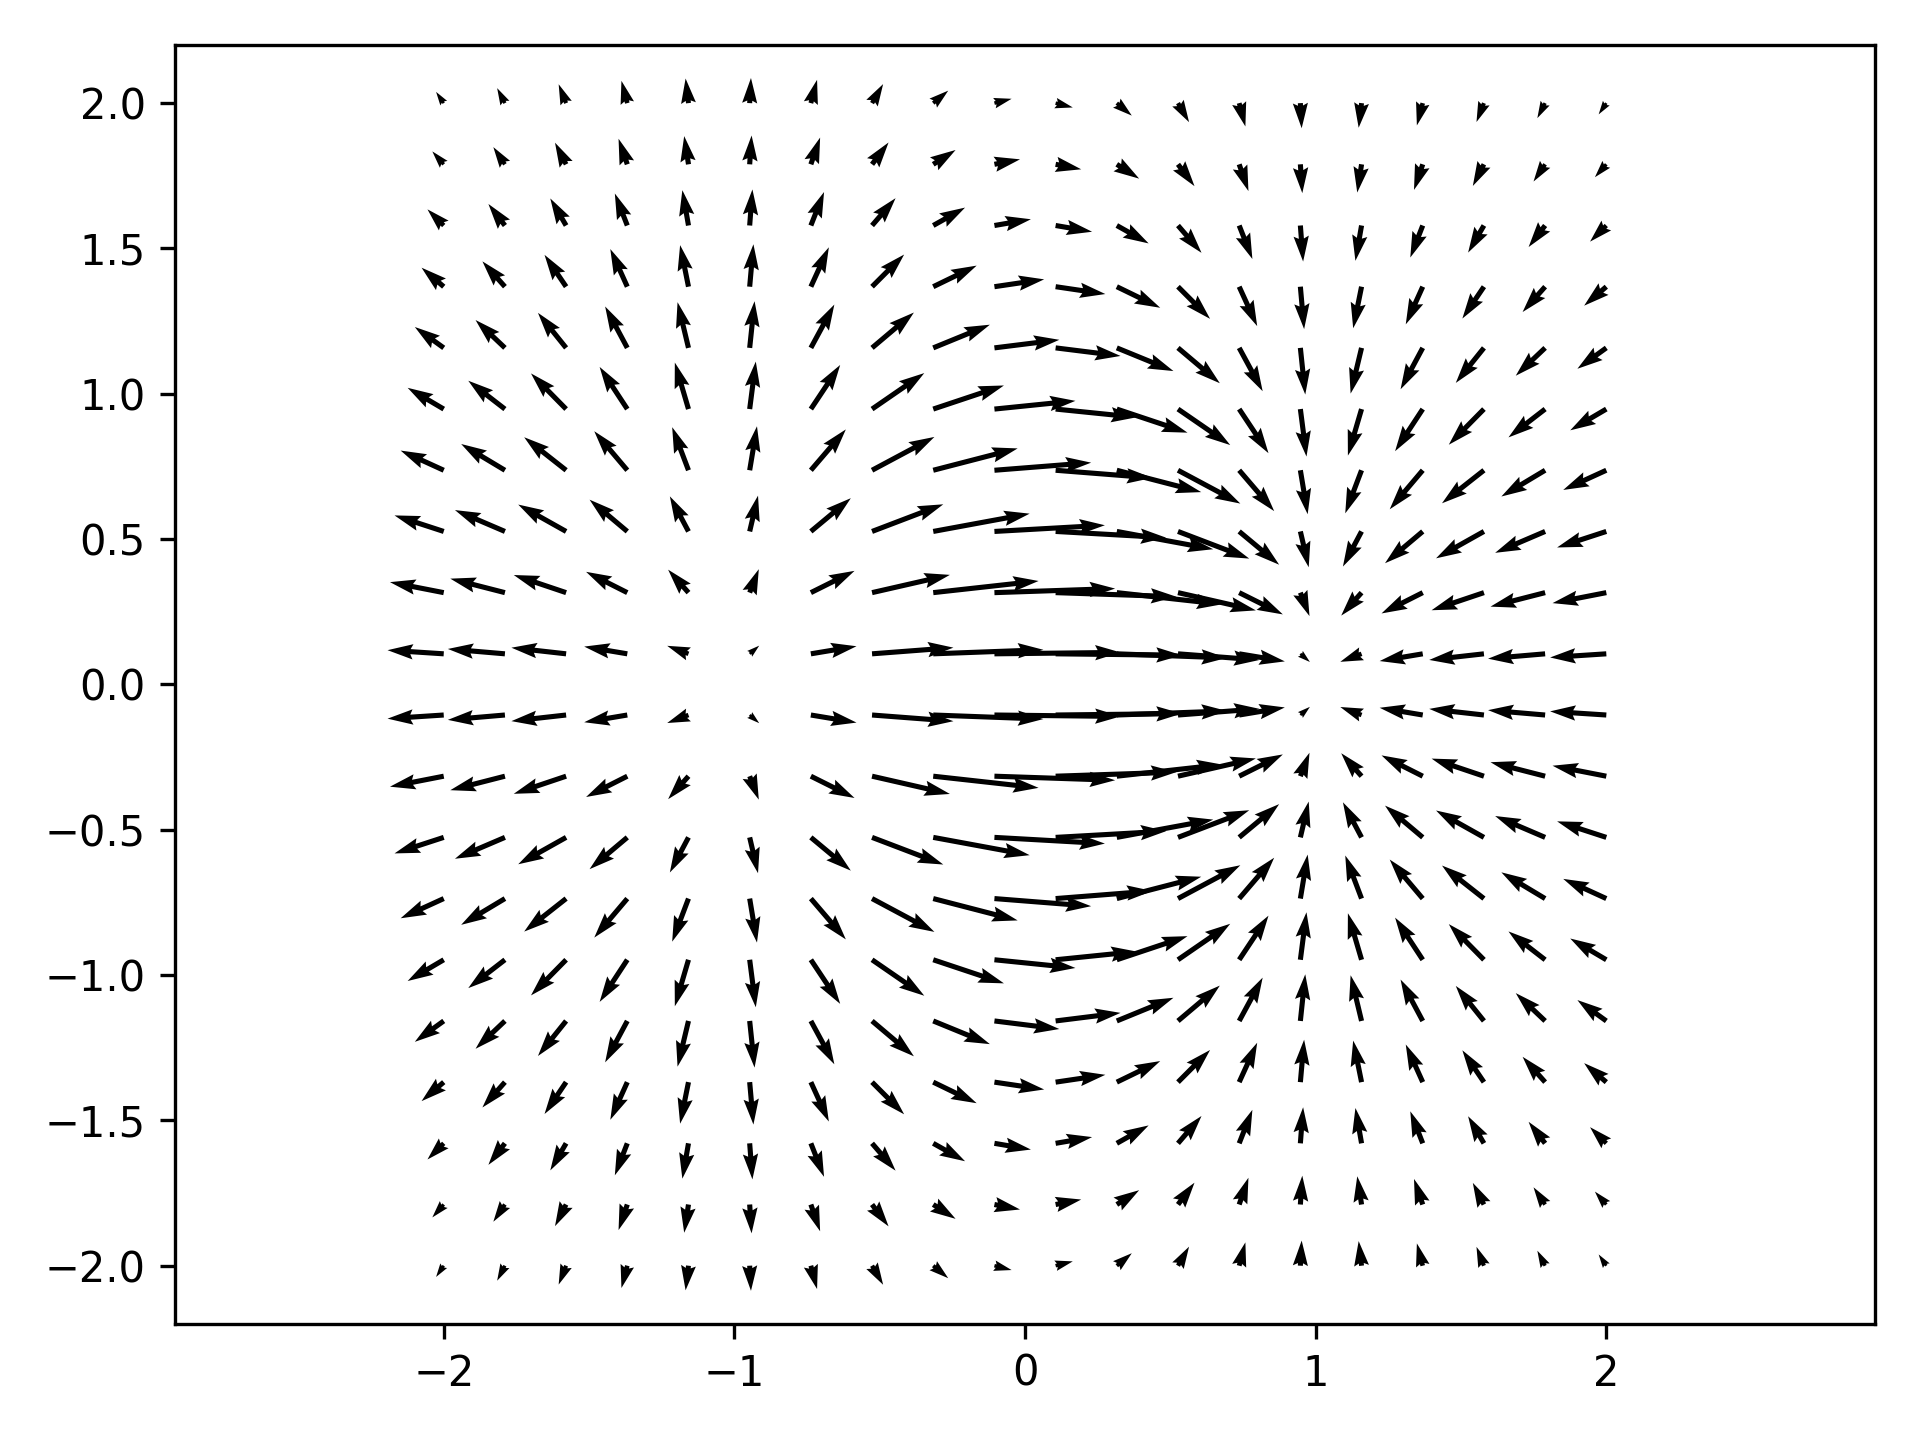
\includegraphics[scale=\myscale,scale=0.6]{figures/fonctions-intro-06}
\end{center}

% dessins 3d voir 'fonctions-intro-06.py'

\end{enumerate}
\end{exemple}


Dans ce chapitre, nous étudions surtout les fonctions $f : \Rr^n \to \Rr$, et plus particulièrement les fonctions $f : \Rr^2 \to \Rr$ ou $f : \Rr^3 \to \Rr$.
Nous reviendrons plus tard sur les fonctions vectorielles $f : \Rr^n \to \Rr^p$.

%----------------------------------------------------
\subsection{Topologie de $\Rr^n$ (rappels/compléments)}

Voici quelques rappels de topologie dans l'espace vectoriel $\Rr^n$. 

\begin{itemize}
  \item Le \defi{produit scalaire} usuel de $x=(x_1,\ldots ,x_n)$ et $y=(y_1,\ldots ,y_n)$, noté $\langle x \mid y\rangle$ (ou bien parfois $x \cdot y$), est défini par
$$\langle x \mid y\rangle = x_1y_1+\dots +x_ny_n.$$

  \item La \defi{norme euclidienne} sur $\Rr^n$ est la norme associée à ce produit scalaire. Pour $x\in \Rr^n$, la norme euclidienne de $x$, notée $\| x\|$, est définie par
$$\| x \| = \sqrt{\langle x \mid x\rangle} = \sqrt{x_1^2+\cdots +x_n^2}.$$

  \item La \defi{distance} entre le point $A = (a_1,\ldots ,a_n)$ et le point $M=(x_1,\dots ,x_n)$ est 
  $$\|M-A\|=\sqrt{(x_1-a_1)^2+\cdots +(x_n-a_n)^2}.$$
  
  \item La \defi{boule ouverte} de centre $A = (a_1,\ldots ,a_n) \in \Rr^n$ et de rayon $r>0$, notée $B_r(A)$, est l'ensemble suivant :
$$B_r(A)=\left\{M\in \Rr^n \mid \|M-A\|<r \right\}.$$


  \item Soient $U$ une partie de $\Rr^n$ et $A\in U$.
On dit que $U$ est un \defi{voisinage} de $A$ si $U$ contient une boule ouverte centrée en $A$.

  \item On dit que $U$ est un \defi{ouvert} de $\Rr^n$ si, pour tout point $A \in U$, $U$ contient une boule ouverte centrée en $A$.
\end{itemize}

Dans le cas de $\Rr^2$, on note plutôt les coordonnées d'un point par $(x,y)$. Alors :
\begin{itemize}
  \item $\langle (x,y) \mid (x',y') \rangle = xx'+yy'$
  \item $\| (x,y) \| = \sqrt{x^2+y^2}$
  \item $B_r(x_0,y_0) = \left\{ (x,y) \in \Rr^2 \mid (x-x_0)^2+(y-y_0)^2 <r^2 \right\}$ (on parle de \defi{disque} plutôt que de boule).
\end{itemize}

De gauche à droite : la norme euclidienne, un disque ouvert, un ouvert $U$.

\myfigure{1}{
  \tikzinput{fig-plusvar-12-01}
  \tikzinput{fig-plusvar-12-02}
  \tikzinput{fig-plusvar-12-03}
} 

Exemples : 
\begin{itemize}
  \item tout rectangle ouvert $]a,b[\times ]c,d[$ est un ouvert de $\Rr^2$ (à droite sur la figure),
  \item tout disque ouvert  de $\Rr^2$ est un ouvert de $\Rr^2$ (à gauche sur la figure).
\end{itemize}
\myfigure{1}{
  \tikzinput{fig-plusvar-12-04}
} 



%%%%%%%%%%%%%%%%%%%%%%%%%%%%%%%%%%%%%%%%%%%%%%%%%%%%%
\section{Graphe}

%----------------------------------------------------
\subsection{Fonctions }

\begin{definition}
Soit $E$ une partie de $\Rr^n$. 
Une \defi{fonction} $f : E \to \Rr$ associe à tout 
$(x_1,\ldots,x_n)$ de $E$ un seul nombre réel $f(x_1,\ldots,x_n)$.
\end{definition}

\begin{exemple}
\sauteligne
\begin{enumerate}
\item Distance d'un point à l'origine en fonction de ses coordonnées :
$$\begin{array}{ccccl}f&:&\Rr^2&\longrightarrow &\Rr\\ &&(x,y)&\longmapsto &\sqrt{x^2+y^2}.\end{array}$$
\item Aire d'un rectangle en fonction de sa longueur et sa largeur :
$$\begin{array}{ccccl}f&:&\Rr^2&\longrightarrow &\Rr\\ &&(x,y)&\mapsto &xy.\end{array}$$
\item Aire d'un parallélépipède en fonction de ses trois dimensions :
$$\begin{array}{ccccl}f&:&\Rr^3&\longrightarrow &\Rr\\ &&(x,y,z)&\mapsto &2(xy+yz+xz).\end{array}$$
\end{enumerate}
\end{exemple}



\begin{definition}
Si on nous donne d'abord une expression pour $f(x_1,\ldots,x_n)$,  alors le \defi{domaine de définition} de $f$ est le plus grand sous-ensemble $D_f \subset \Rr^n$ tel que, pour chaque $(x_1,\ldots,x_n)$ de $D_f$, $f(x_1,\ldots,x_n)$ soit bien définie. La fonction est alors $f : D_f \to \Rr$.
\end{definition}


\begin{exemple}
\sauteligne
\begin{enumerate}
  \item $f(x,y) = \ln(1 + x + y)$

  Il faut que $1+x+y$ soit strictement positif, afin de pouvoir calculer son logarithme. Donc :
  $$D_f = \left\{ (x,y)\in \Rr^2 \mid 1+x+y >0 \right\}$$
  
  Pour tracer cet ensemble, on trace d'abord la droite  d'équation $1+x+y=0$. On détermine ensuite de quel côté de la droite est l'ensemble $1+x+y>0$. Ici, c'est au-dessus de la droite.
  
\myfigure{0.5}{
    \tikzinput{fig-plusvar-101}
}  

  \item $f(x,y) = \exp\left(\frac{x+y}{x^2-y}\right)$
  
  Le dénominateur ne doit pas s'annuler :  
  $$D_f = \left\{ (x,y)\in \Rr^2 \mid x^2-y \neq 0 \right\}$$
  
  Les points de l'ensemble de définition sont tous les points du plan qui ne sont pas sur la parabole d'équation $(y=x^2)$.
  
\myfigure{0.6}{
    \tikzinput{fig-plusvar-102}
}

  \item $f(x,y,z) = \frac {1}{\sqrt{x^2 + y^2 + z^2 - 2}}$
  
   L'expression sous la racine doit être positive (pour pouvoir prendre la racine carrée) et ne doit pas s'annuler (pour pouvoir prendre l'inverse). Donc :
  $$D_f = \left\{ (x,y,z)\in \Rr^3 \mid x^2+y^2+z^2 > 2 \right\}$$
  Autrement dit, ce sont tous les points en dehors de la boule fermée centrée en $(0,0,0)$ et de rayon $\sqrt 2$.
  
\myfigure{0.8}{
    \tikzinput{fig-plusvar-103}
}
      
  
\end{enumerate}
\end{exemple}



\begin{definition}
L'\defi{image} d'une fonction $f : E \to \Rr$ est l'ensemble des valeurs $f(x_1,\ldots,x_n)$ prises par $f$ lorsque $(x_1,\ldots,x_n)$ parcourt $E$ :
$$\Im f = \big\{ f(x_1,\ldots,x_n) \mid (x_1,\ldots,x_n) \in E \big\} \subset \Rr$$
\end{definition}

\begin{exemple}
\sauteligne
\begin{enumerate}
  \item $f(x,y) = \ln(1 + x + y)$

  L'image de $f$ est $\Rr$ tout entier : $\Im f = \Rr$.
  
  Preuve : soit $z\in\Rr$. Alors, pour $(x,y) = (e^z,-1) \in D_f$, on a 
  $$f(x,y)= f(e^z,-1) = \ln(e^z)=z.$$ 
  Donc tout $z\in\Rr$ est dans l'image de $f$.
  
  \item $f(x,y) = \exp\left(\frac{x+y}{x^2-y}\right)$
 
  $\Im f = {}]0,+\infty[$.
  
  Preuve : On a bien sûr $f(x,y)>0$ pour tout $(x,y) \in D_f$.
 Réciproquement, soit $z\in {}]0,+\infty[$. 
  Si $z \neq 1$ alors, pour $(x,y)=(\tfrac{1}{\ln z},0) \in D_f$, on a 
  $$f(x,y)= f(\tfrac{1}{\ln z},0) = \exp\left(\frac{\tfrac{1}{\ln z}}{(\tfrac{1}{\ln z})^2}\right)= \exp(\ln z) = z.$$ 
 Si $z = 1$ alors, pour $(x,y)=(1,-1) \in D_f$, on a 
  $f(x,y)= f(1,-1) = \exp(0)= 1$.
    
  \item Pour $f(x,y,z) = \frac {1}{\sqrt{x^2 + y^2 + z^2 - 2}}$, on a
  $\Im f = {}]0,+ \infty[$.
  À vous de faire la preuve !
 
  
\end{enumerate}
\end{exemple}


\begin{definition}
Soit $E$ une partie de $\Rr^n$. 
Une \defi{fonction vectorielle} $f : E \to \Rr^p$ associe à tout 
$(x_1,\ldots,x_n)$ de $E$ un $p$-uplet de nombres réels.
On la note 
$$\begin{array}{ccccl}f&:&\Rr^n&\longrightarrow &\Rr^p\\ &&x&\longmapsto &\left(f_1(x),f_2(x),\ldots ,f_p(x)\right).\end{array}$$
\end{definition}


Nous nous limiterons souvent aux dimensions inférieures ou égales à $3$ pour $n$ et $p$, la généralisation aux dimensions supérieures ne posant pas de problème particulier, sauf pour faire des dessins. Voici quelques exemples simples.

\begin{exemple}
\sauteligne
\begin{enumerate}
\item Aire et volume d'un parallélépipède rectangle en fonction de ses trois dimensions :
$$\begin{array}{ccccl}f&:&\Rr^3& \longrightarrow &\Rr^2\\ &&(x,y,z)&\longmapsto &\big(2(xy+yz+xz),xyz\big).\end{array}$$

\item Coordonnées polaires d'un point du plan :
$$\begin{array}{ccccl}f&:&\Rr_+\times [0,2\pi[&\longrightarrow &\Rr^2\\ &&(r,\theta)&\longmapsto &(r\cos \theta ,r\sin \theta ).\end{array}$$
\end{enumerate}
\end{exemple}



%----------------------------------------------------
\subsection{Graphe et lignes de niveau}



\begin{definition}
Soit $f : D_f \subset \Rr^2 \to \Rr$ une fonction de $2$ variables. 
Le \defi{graphe} $\mathcal{G}_f$ de $f$ est le sous-ensemble de $\Rr^3$ formé des points de coordonnées $(x,y,f(x,y))$ avec $(x,y)$ dans l'ensemble de définition. Le graphe est donc :
$$\mathcal{G}_f= \big\{ (x,y,z)\in \Rr^3 \mid (x,y)\in D_f \text{ et } z=f(x,y)\big\}.$$
\end{definition}

Représenter graphiquement le graphe n'est possible que pour les fonctions d'une seule variable ou de deux variables. 
Pour les fonctions d'une variable $f: D_f \subset \Rr \to \Rr$, on rappelle que le graphe est 
$$\mathcal{G}_f = \big\{ (x,y)\in \Rr^2 \mid x \in D_f \text{ et } y=f(x)\big\}.$$


Dans le cas d'une variable (à gauche), le graphe est une courbe ; dans le cas de deux variables qui nous intéresse ici, c'est une surface.

\begin{center}
\begin{minipage}{0.4\textwidth}
\myfigure{0.7}{
    \tikzinput{fig-plusvar-104}   
}
\end{minipage}
\begin{minipage}{0.4\textwidth}
\myfigure{0.5}{
    \tikzinput{fig-plusvar-105}   
}\end{minipage}
\end{center}

Afin de tracer le graphe d'une fonction de deux variables, on découpe la surface en morceaux.


\bigskip

\evidence{Tranches.}

Une première façon de faire : tracer, pour quelques valeurs de $a$ et $b$, les graphes des fonctions partielles
$$f_1:x\mapsto f(x,b) \quad \text{ et } \quad f_2:y\mapsto f(a,y).$$
La première représente l'intersection du graphe $\mathcal{G}_f$ avec le plan $(y=b)$ \couleurnb{(en orange) }{} et la seconde représente l'intersection du graphe avec le plan $(x=a)$ \couleurnb{(en vert)}{}.

\myfigure{0.7}{
    \tikzinput{fig-plusvar-106} \qquad  
    \tikzinput{fig-plusvar-107}      
}


\bigskip

\evidence{Lignes de niveau.}

On va aussi s'intéresser à d'autres courbes tracées sur la surface : les courbes de niveau.


\begin{definition}

Soit $f : D_f \subset \Rr^2 \to \Rr$ une fonction de deux variables. 
\begin{itemize}
  \item La \defi{ligne de niveau} 
$z=c\in \Rr$ est 
$$L_c =\big\{(x,y)\in D_f \mid f(x,y)=c \big\}.$$
  \item La \defi{courbe de niveau} $z=c$ est la trace de $\mathcal{G}_f$ dans le plan $(z=c)$ : 
$$\mathcal{G}_f \cap (z=c) = \big\{ (x,y,c)\in \Rr^3 \mid f(x,y)=c \big\}.$$
\end{itemize}
\end{definition}


La ligne de niveau $c$ est une courbe du plan $\Rr^2$, la courbe de niveau $c$
est une courbe de l'espace $\Rr^3$. On obtient la courbe de niveau $c$ en partant de la ligne de niveau $c$ et en remontant à l'altitude $c$.

\begin{exemple}
Soit $f : \Rr^2 \to \Rr$ définie par $f(x,y)=x^2+y^2$. 

  \begin{itemize}
    \item Si $c<0$, la ligne de niveau $L_c$ est vide (aucun point n'a d'altitude négative).
    \item Si $c=0$, la ligne de niveau $L_0$ se réduit à $\{(0,0)\}$.
    \item Si $c>0$, la ligne de niveau $L_c$  est le cercle du plan de centre $(0,0)$ et de rayon $\sqrt{c}$. On remonte $L_c$ à l'altitude $z=c$ : la courbe de niveau est alors le cercle horizontal de l'espace de centre $(0,0,c)$ et de rayon $\sqrt{c}$. 
  \end{itemize}
      
Le graphe est alors une superposition de cercles horizontaux de l'espace de centre $(0,0,c)$ et de rayon $\sqrt{c}$ avec $c \ge 0$.     

Ci-dessous : (a) le graphe, appelé paraboloïde de révolution, (b) $5$ courbes de niveau, (c) $10$ courbes de niveau, (d) des lignes de niveau dans le plan.
\begin{center}
    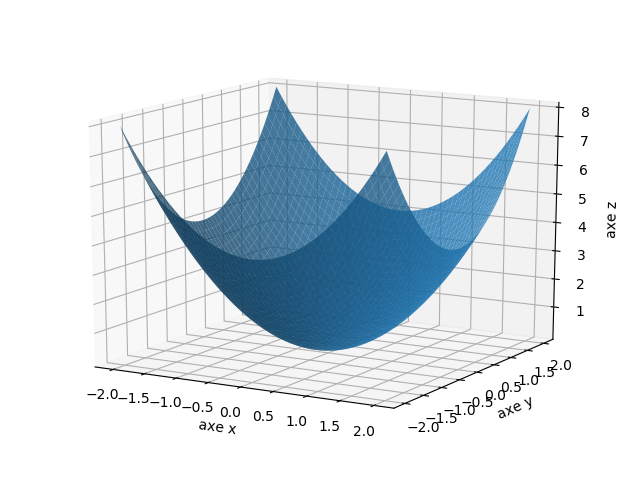
\includegraphics[scale=\myscale,scale=0.5]{figures/fonctions-niveau-1a}
    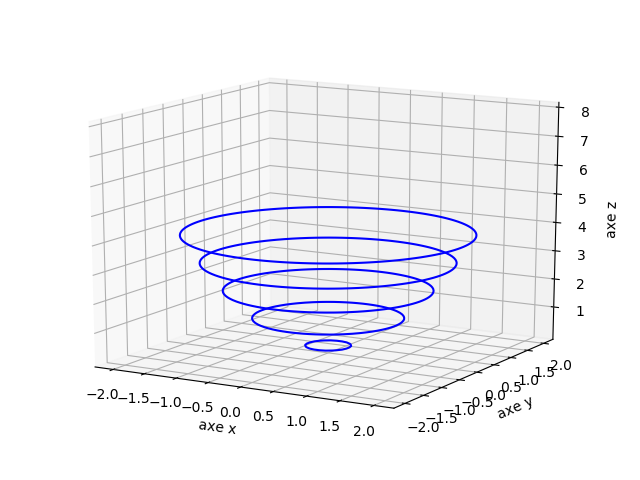
\includegraphics[scale=\myscale,scale=0.5]{figures/fonctions-niveau-1b}
    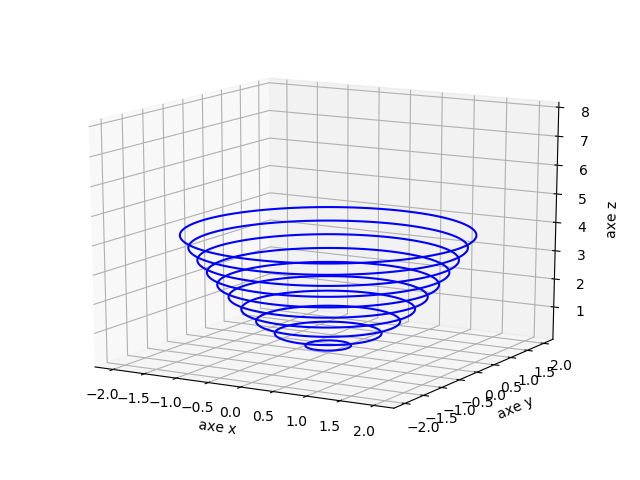
\includegraphics[scale=\myscale,scale=0.5]{figures/fonctions-niveau-1c}
    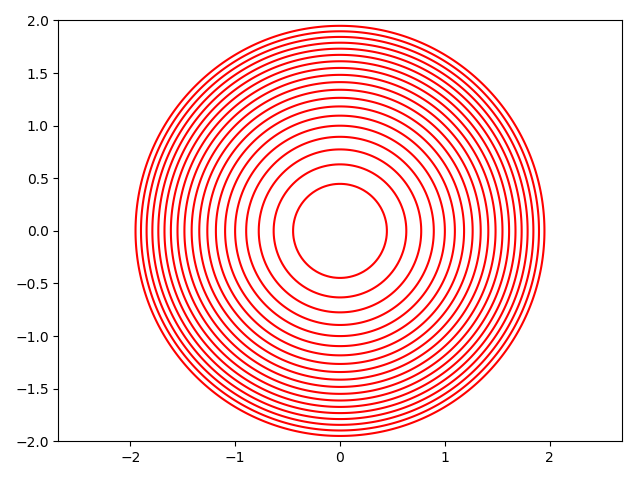
\includegraphics[scale=\myscale,scale=0.5]{figures/fonctions-niveau-1d}
\end{center}

% dessins 3d voir 'fonctions-niveau-1.py'
\end{exemple}



\begin{exemple}
Sur une carte topographique, les lignes de niveau représentent les courbes ayant la même altitude. 
\begin{center}
  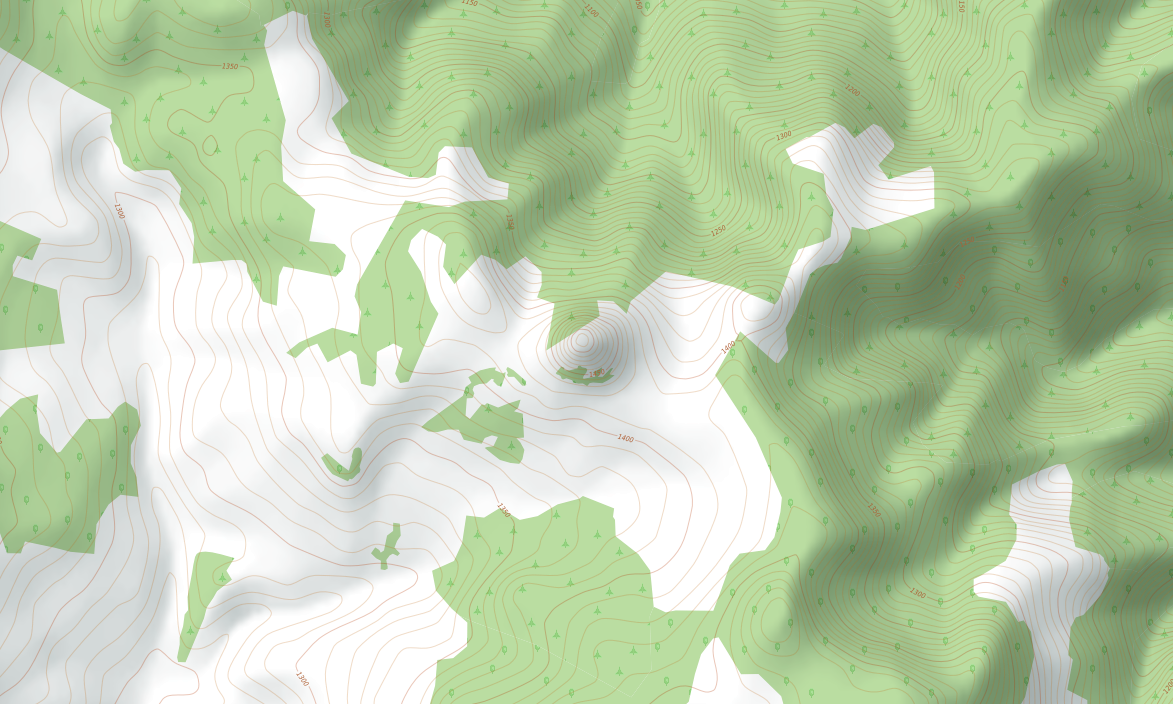
\includegraphics[scale=\myscale,scale=0.4]{figures/fig-plusvar-topo}
\end{center}
\begin{itemize}
  \item Ici, une carte \emph{Open Street Map} avec, au centre, le mont Gerbier-de-Jonc (source de la Loire, 1551 m). 
  \item Les lignes de niveau correspondent à des altitudes par cran de $10$ m (par exemple, pour $c=1400$, $c=1410$, $c=1420$\ldots).
  \item Lorsque les lignes de niveau sont très espacées, le terrain est plutôt plat ; lorsque les lignes sont rapprochées, le terrain est pentu.
  \item Par définition, si on se promène en suivant une ligne de niveau, on reste toujours à la même altitude !
\end{itemize}
\end{exemple}


\begin{exemple}
L'image qui a servi lors de l'introduction est le graphe et les lignes de niveau de la fonction $f : \Rr^2 \to \Rr$ définie par
$$(x,y) \mapsto z = 
\frac{\sin \left( x^{2}+3y^{2} \right)}{\frac{1}{10}+r^{2}}+\left( x^{2}+5y^{2} \right)\cdot \frac{\exp \left( 1-r^{2} \right)}{2} \quad \text{ avec } \quad r=\sqrt{x^{2}+y^{2}}.$$
%Les courbes de niveau, sont projetées sur les plans $z=0$ et $z=9$ pour donner les lignes de niveau.

\begin{center}
%    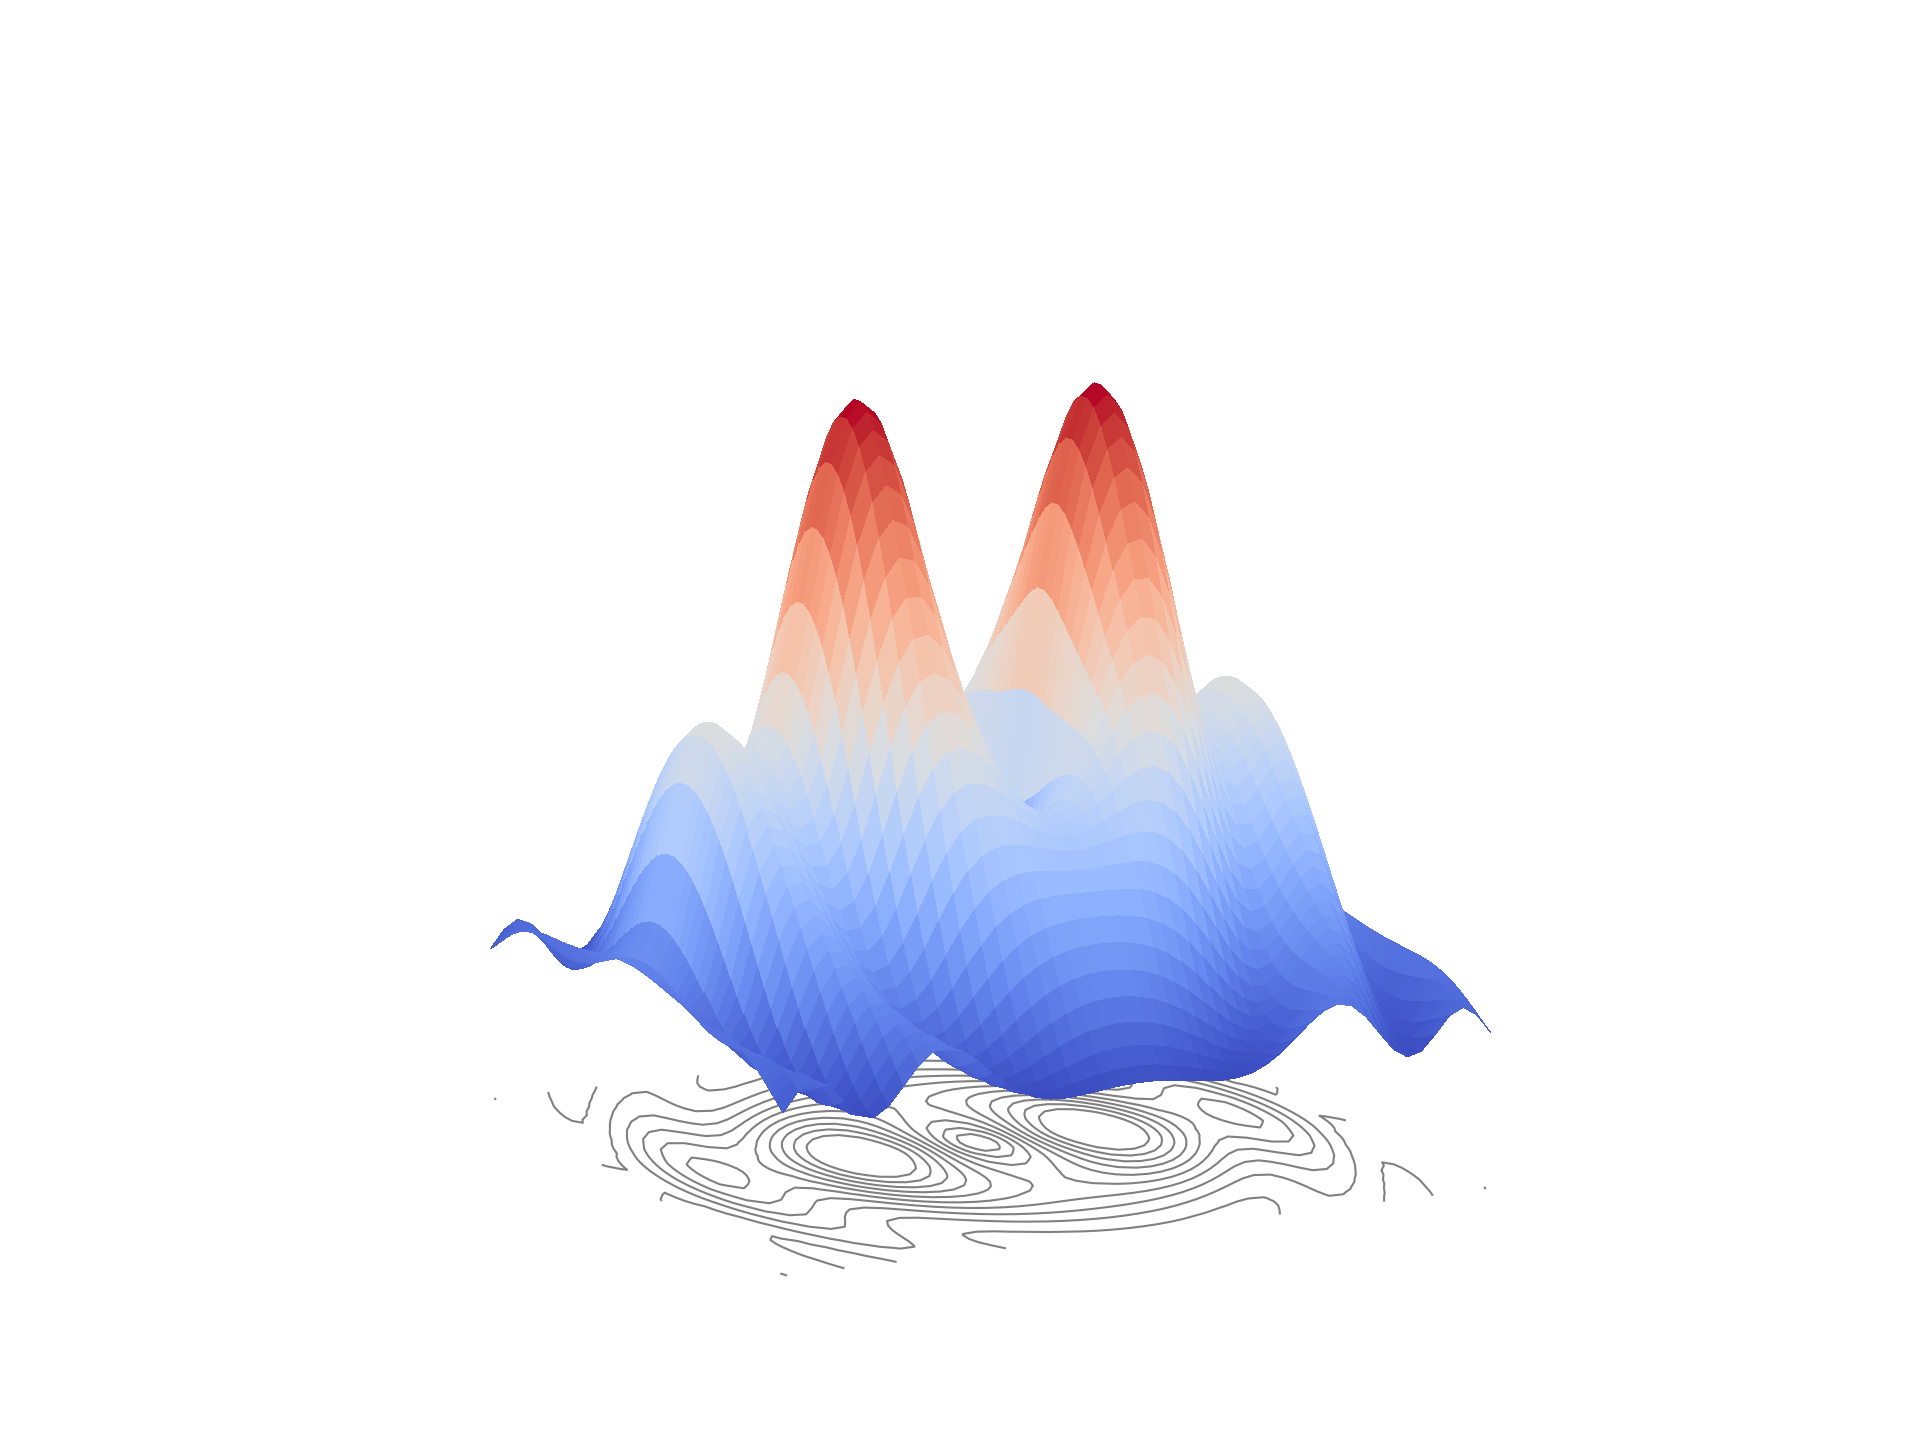
\includegraphics[scale=\myscale,scale=0.5]{figures/fonctions-niveau-3a}
    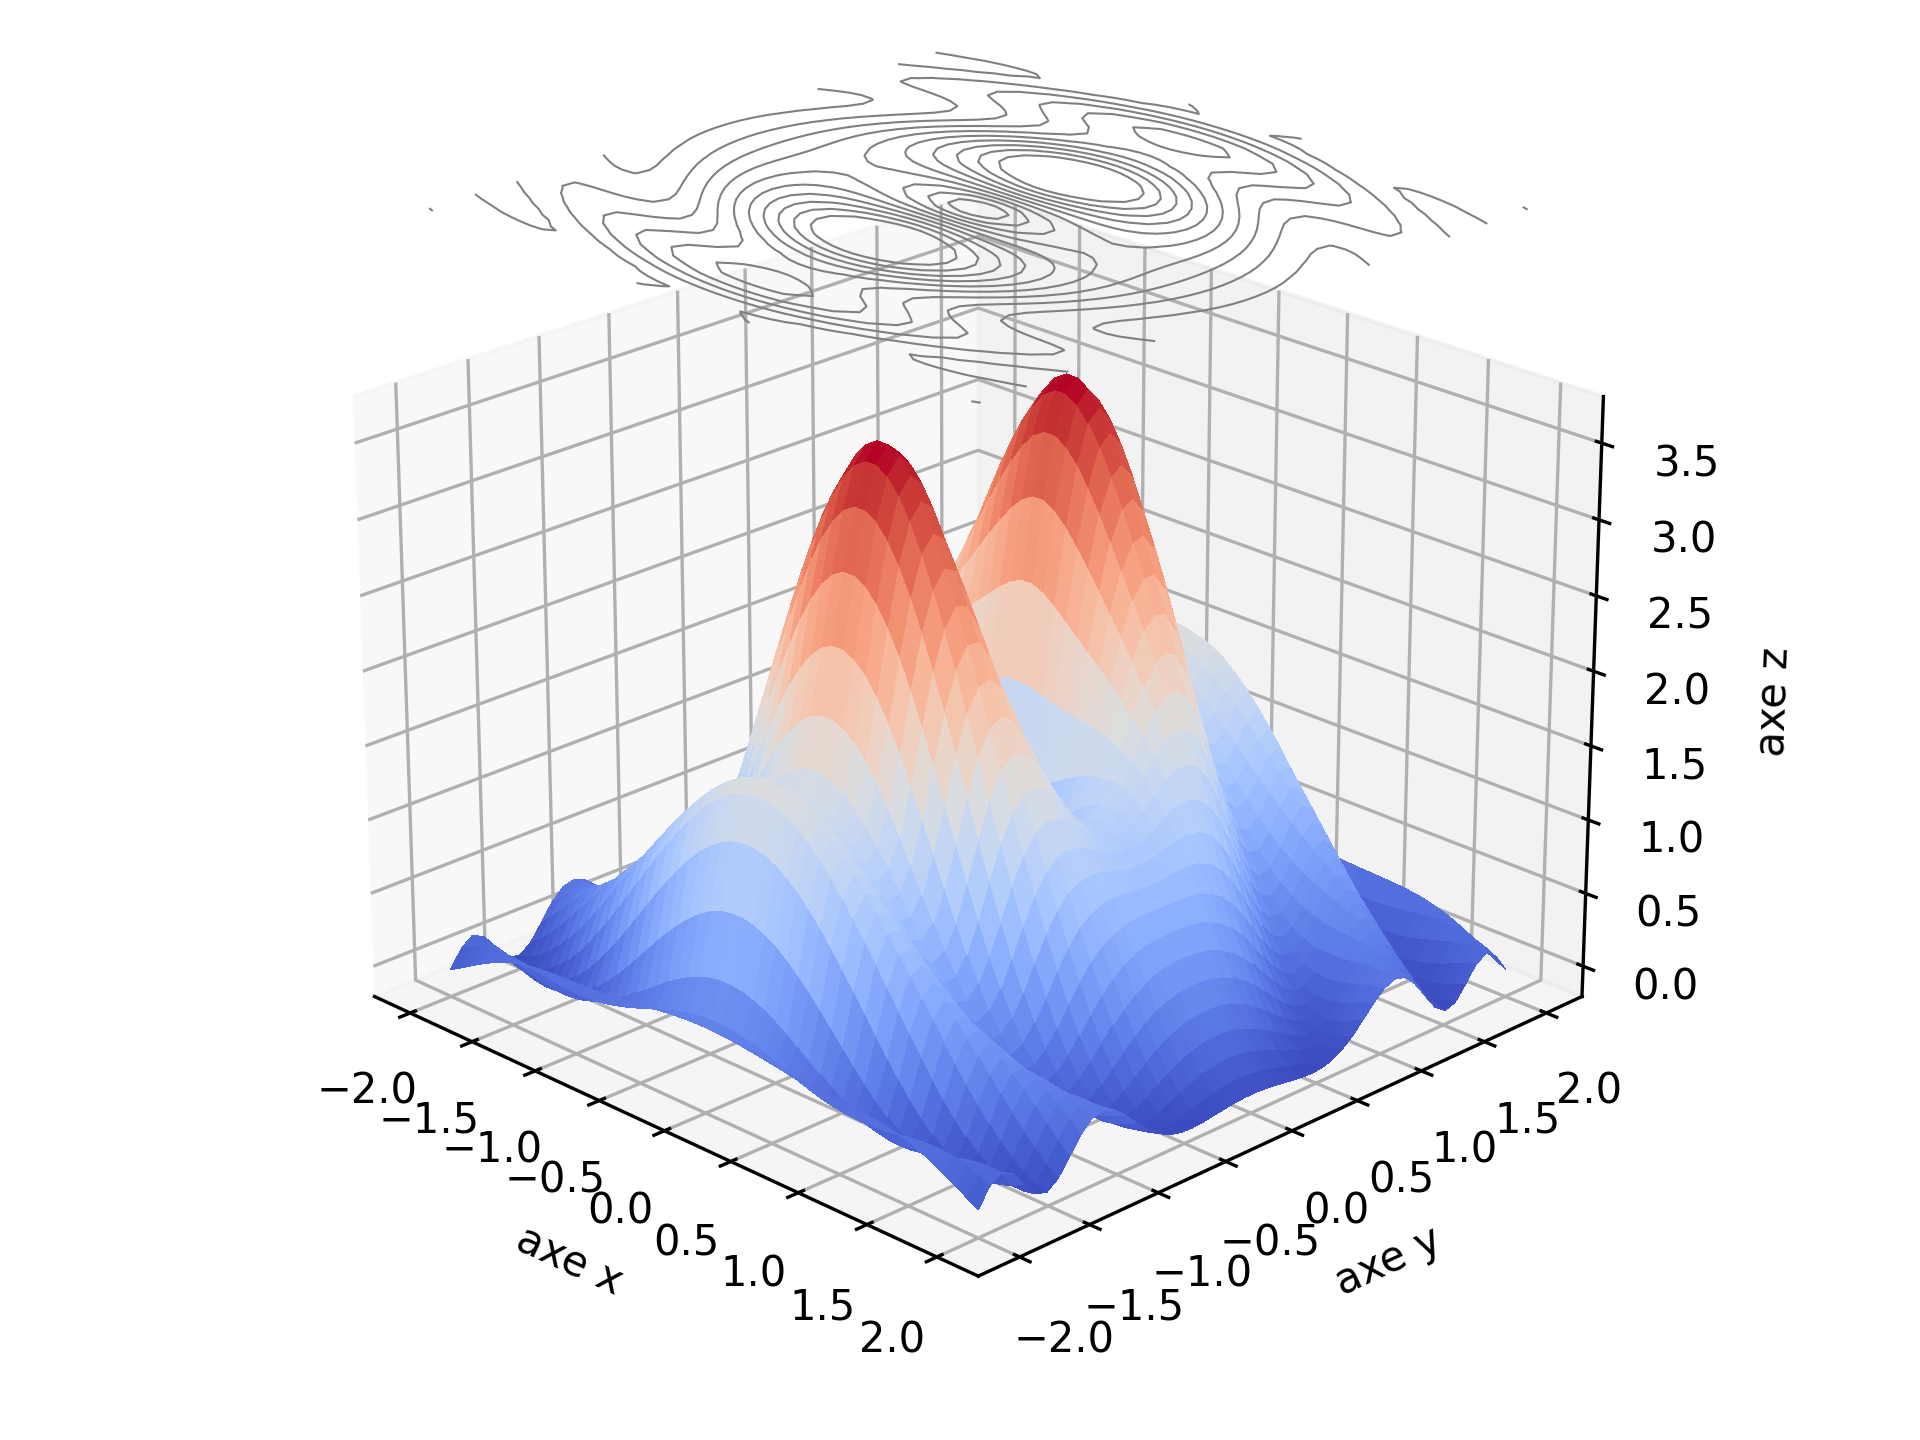
\includegraphics[scale=\myscale,scale=0.5]{figures/fonctions-niveau-3c}
    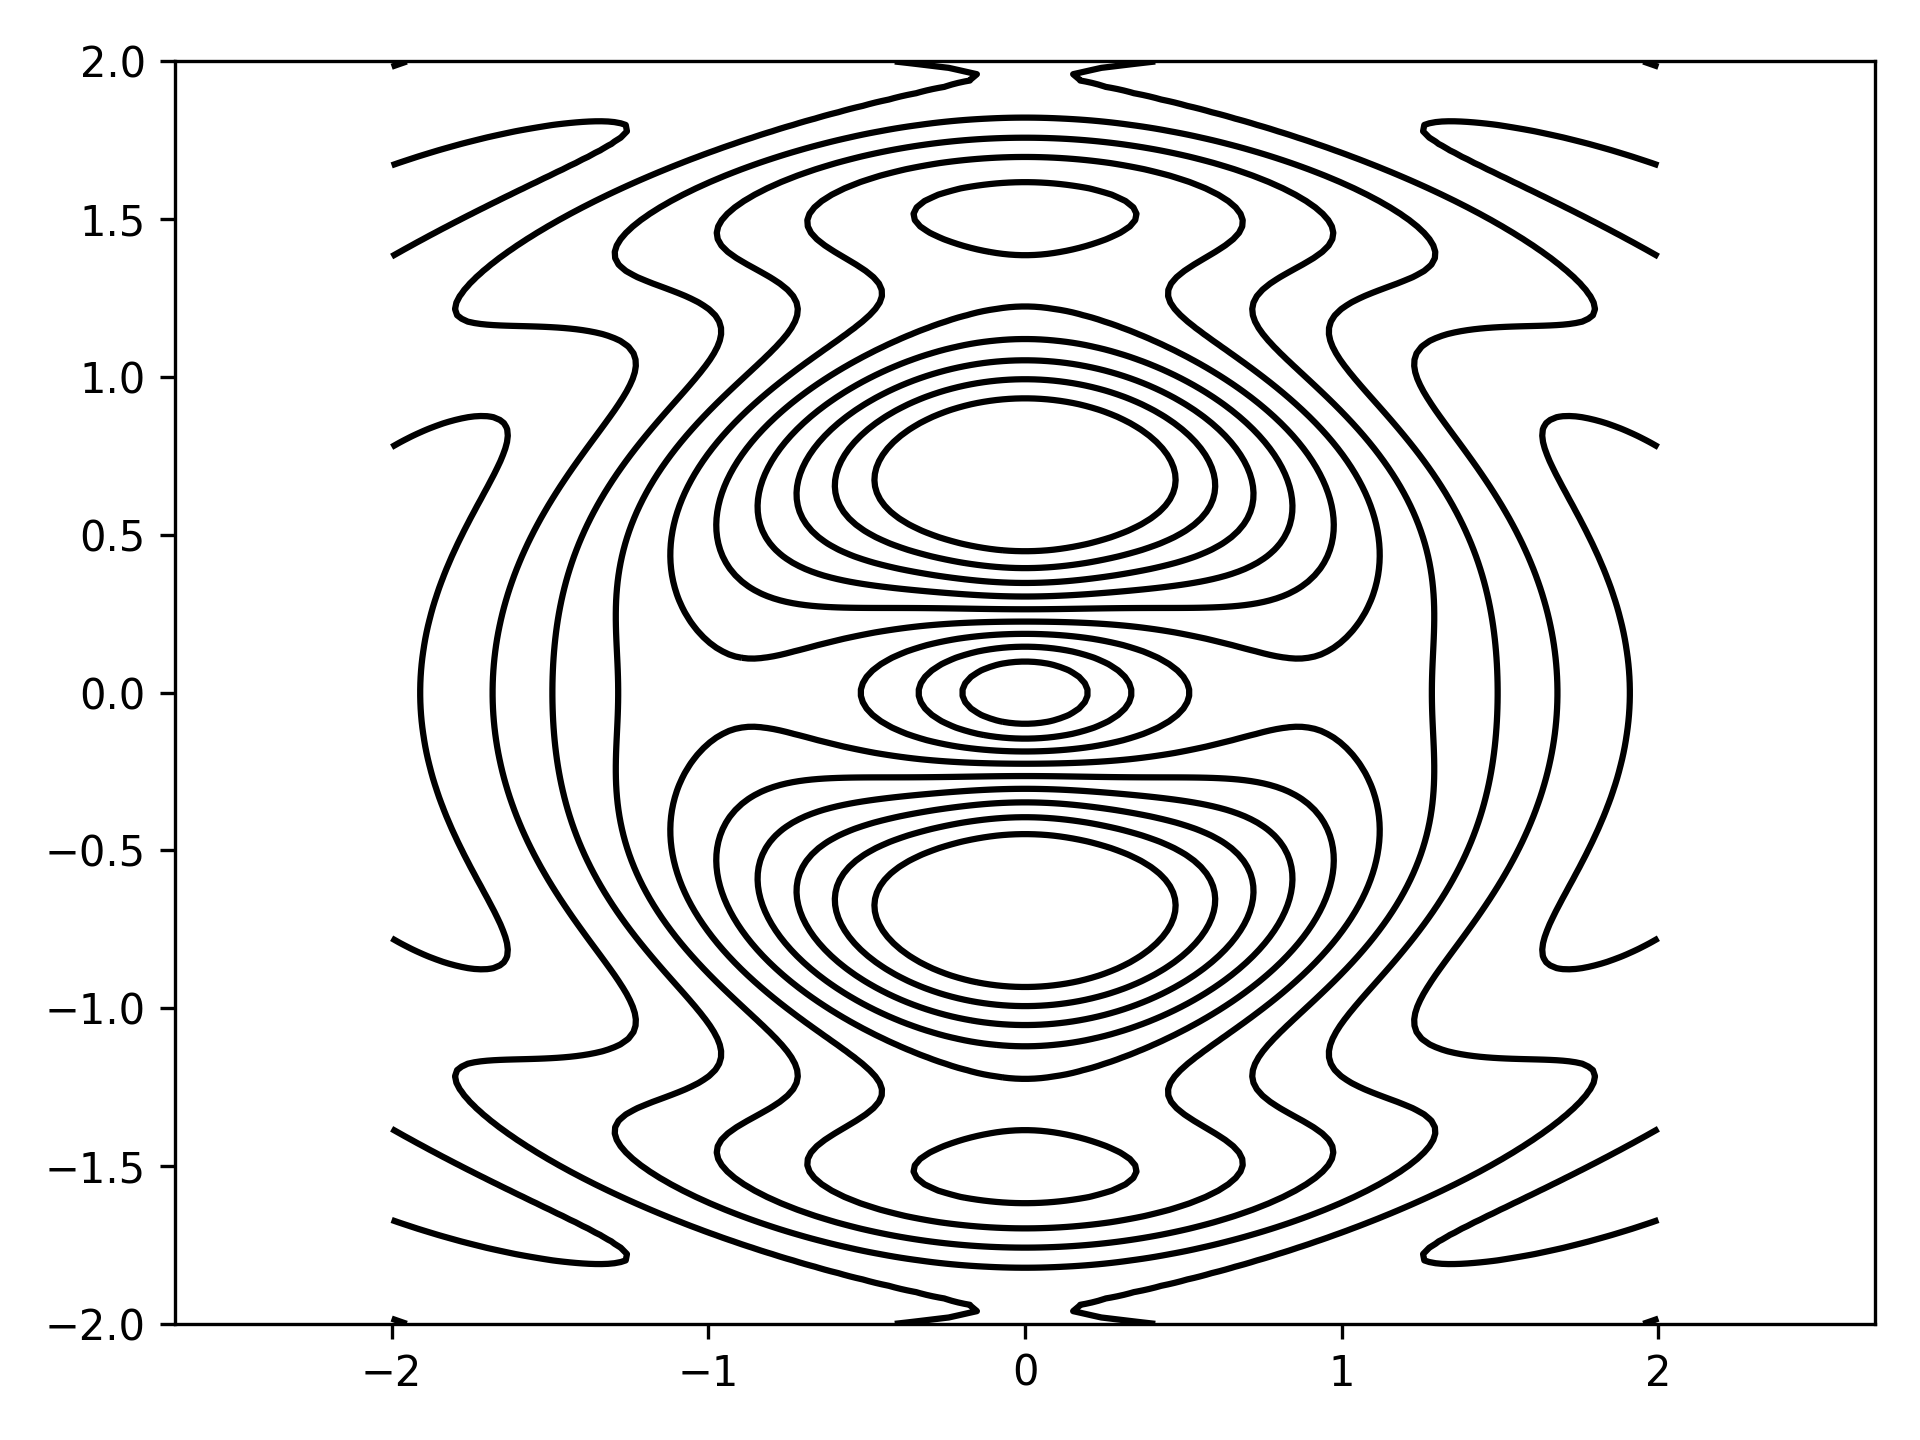
\includegraphics[scale=\myscale,scale=0.5]{figures/fonctions-niveau-3b}
\end{center}

% dessins 3d voir 'fonctions-niveau-3.py'


\end{exemple}   

 
 
\bigskip

\evidence{Surfaces de niveau.}

Pour les fonctions de $3$ variables, le graphe étant dans $\Rr^4$, on ne peut le dessiner. 
La notion analogue à la ligne de niveau est celle de \defi{surface de niveau}, donnée par l'équation $f(x,y,z)=c$.


\begin{exemple}
$f(x,y,z) = x^2+y^2+z^2$. Les surfaces de niveau sont données par l'équation $x^2+y^2+z^2=c$. 
Pour $c \ge 0$, ces surfaces sont des sphères, centrées à l'origine et de rayon $\sqrt{c}$. 
Voici ces surfaces pour $c=1,3,5$. Elles ont été découpées pour laisser entrevoir les surfaces des différents niveaux.

\begin{center}
    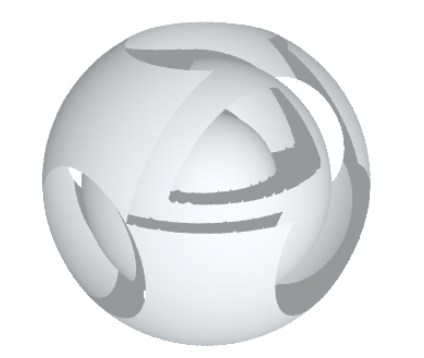
\includegraphics[scale=\myscale,scale=0.5]{figures/surface-niveau}
\end{center}

% dessins 3d voir 'surface-niveau.sage'
\end{exemple}



\subsection{Exemples de surfaces quadratiques}

Ce sont des exemples à connaître, car ils seront fondamentaux pour la suite du cours.

\begin{exemple}
$$f(x,y) = \frac{x^2}{a^2} + \frac{y^2}{b^2}-1$$

\begin{itemize}
  \item Les tranches sont des paraboles.
  \item Les lignes de niveau sont des ellipses.
  \item Le graphe est donc un \defi{paraboloïde elliptique}.
\end{itemize}

Ci-dessous : (a) la surface, (b) des tranches avec $x$ constant, (c) des tranches avec $y$ constant, (d) des courbes de niveau, (e) des lignes de niveau dans le plan.

\begin{center}
    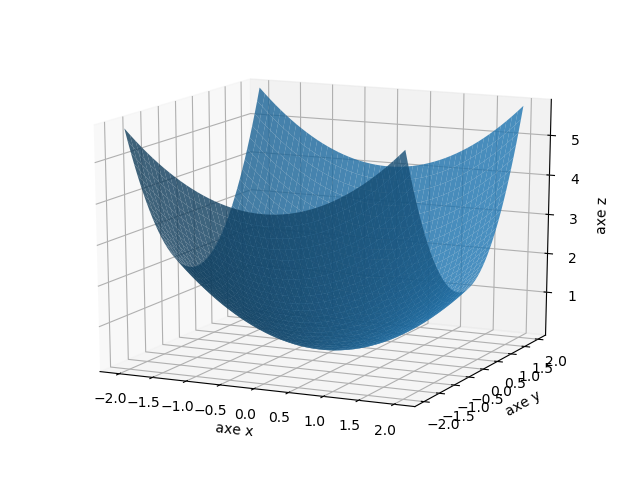
\includegraphics[scale=\myscale,scale=0.5]{figures/fonctions-quadra-1a}
    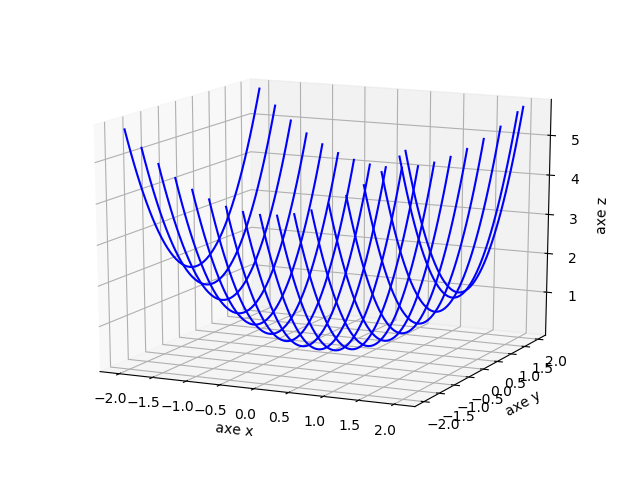
\includegraphics[scale=\myscale,scale=0.5]{figures/fonctions-quadra-1b}
    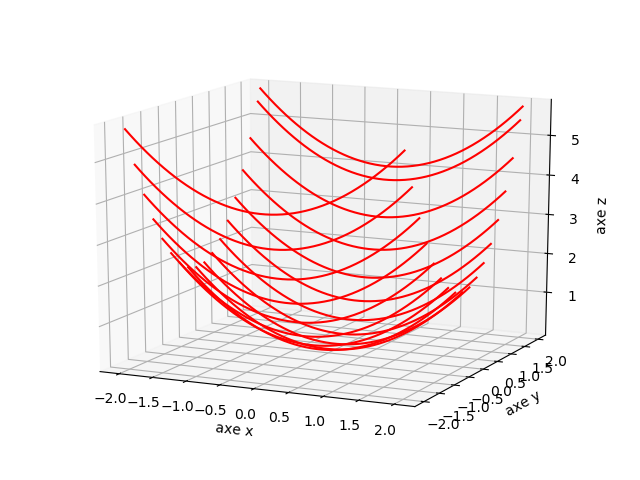
\includegraphics[scale=\myscale,scale=0.5]{figures/fonctions-quadra-1c}
    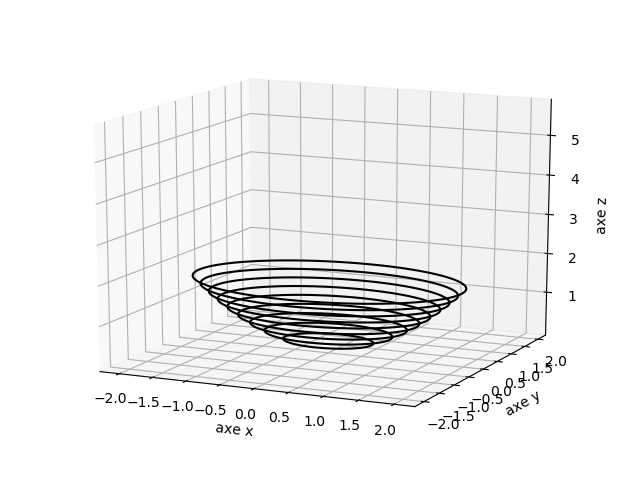
\includegraphics[scale=\myscale,scale=0.5]{figures/fonctions-quadra-1d}
    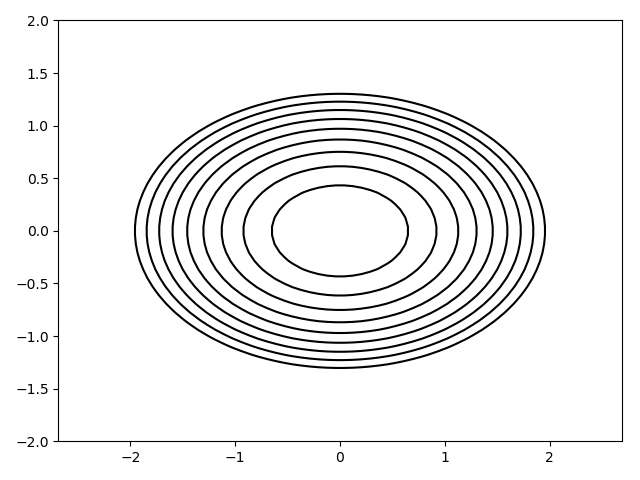
\includegraphics[scale=\myscale,scale=0.5]{figures/fonctions-quadra-1e}
\end{center}

% dessins 3d voir 'fonctions-quadra-1.py' 

\end{exemple}


\begin{exemple}
$$f(x,y) = x^2$$

\begin{itemize}
  \item Les tranches (à $y$ constant) sont des paraboles.
  \item Les lignes de niveau sont des paires de droites.
  \item Le graphe est donc un \defi{cylindre parabolique}.
\end{itemize}


Ci-dessous : (a) la surface, (b) des tranches avec $x$ constant, (c) des tranches avec $y$ constant, (d) des courbes de niveau, (e) des lignes de niveau dans le plan.
\begin{center}
    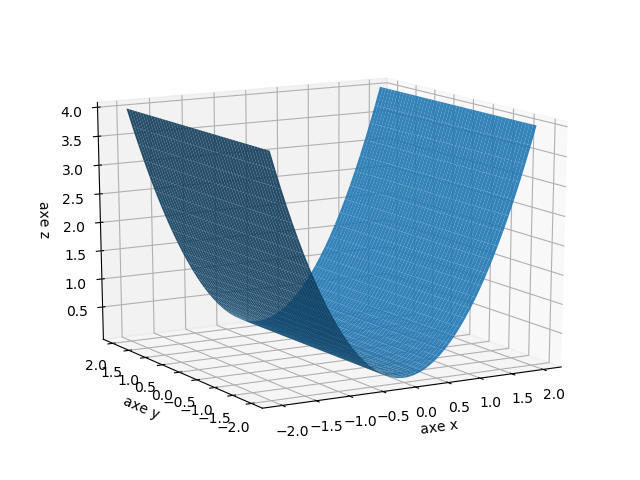
\includegraphics[scale=\myscale,scale=0.5]{figures/fonctions-quadra-2a}
    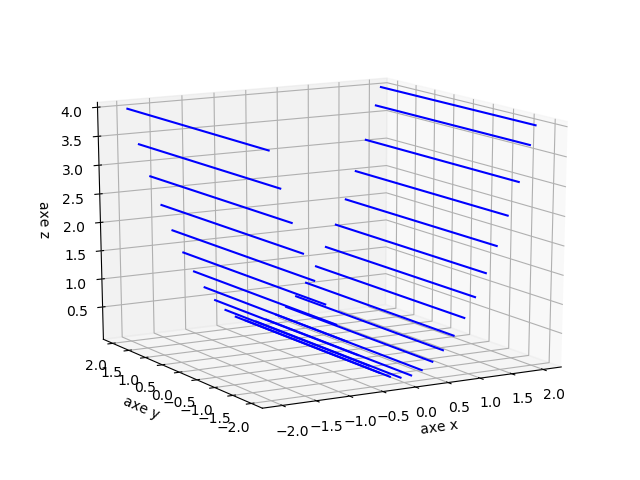
\includegraphics[scale=\myscale,scale=0.5]{figures/fonctions-quadra-2b}
    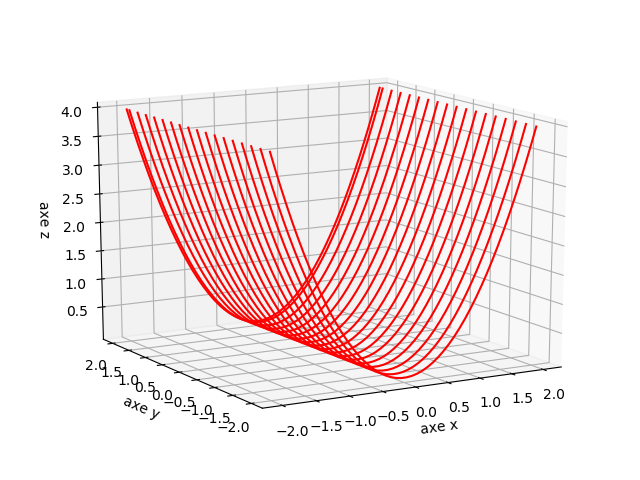
\includegraphics[scale=\myscale,scale=0.5]{figures/fonctions-quadra-2c}
    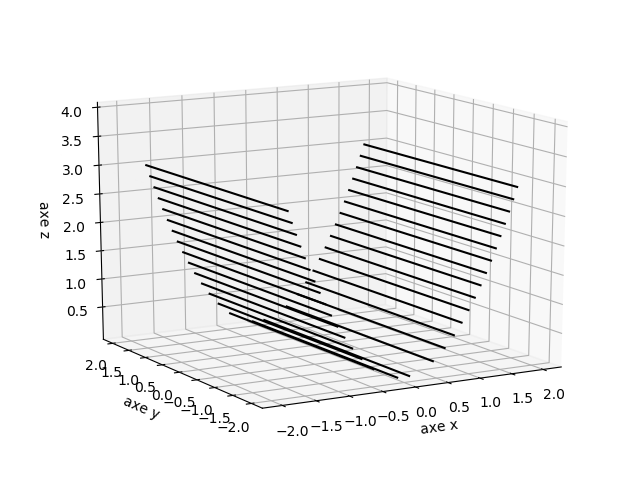
\includegraphics[scale=\myscale,scale=0.5]{figures/fonctions-quadra-2d}
    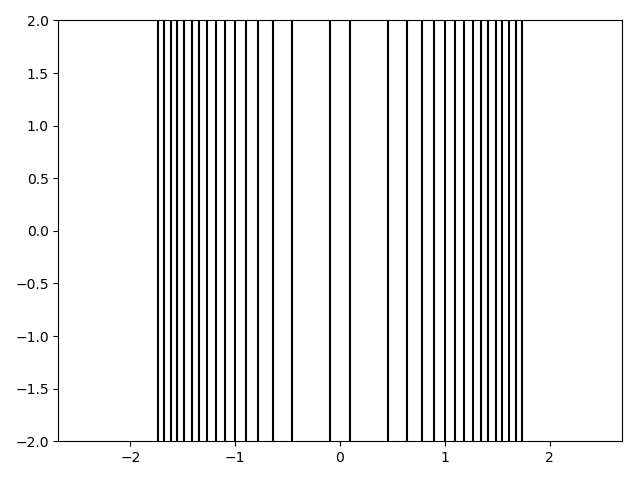
\includegraphics[scale=\myscale,scale=0.5]{figures/fonctions-quadra-2e}
\end{center}

% dessins 3d voir 'fonctions-quadra-2.py' 

\end{exemple}


\begin{exemple}
$$f(x,y) = x^2-y^2$$

\begin{itemize}
  \item Les tranches sont des paraboles.
  \item Les lignes de niveau sont des hyperboles.
  \item Le graphe est donc un \defi{paraboloïde hyperbolique}, que l'on appelle aussi la \defi{selle de cheval}.
  \item Un autre nom pour cette surface est un \defi{col} (du nom d'un col de montagne). 
  En effet, le point $(0,0,0)$ est le point de passage le moins haut pour passer d'un versant à l'autre de la montagne. 
\end{itemize}


Ci-dessous : (a) la surface, (b) des tranches avec $x$ constant, (c) des tranches avec $y$ constant, (d) des courbes de niveau, (e) des lignes de niveau dans le plan (en pointillé les lignes de niveau négatif).
\begin{center}
    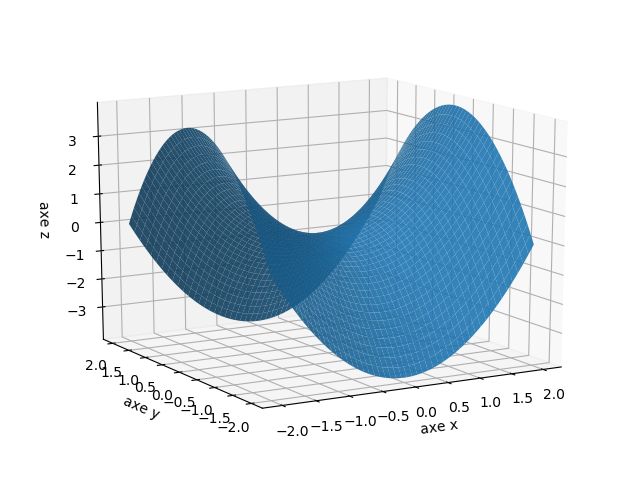
\includegraphics[scale=\myscale,scale=0.5]{figures/fonctions-quadra-3a}
    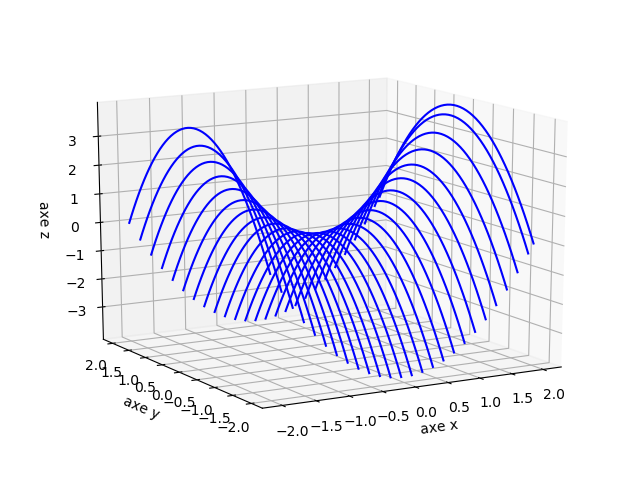
\includegraphics[scale=\myscale,scale=0.5]{figures/fonctions-quadra-3b}
    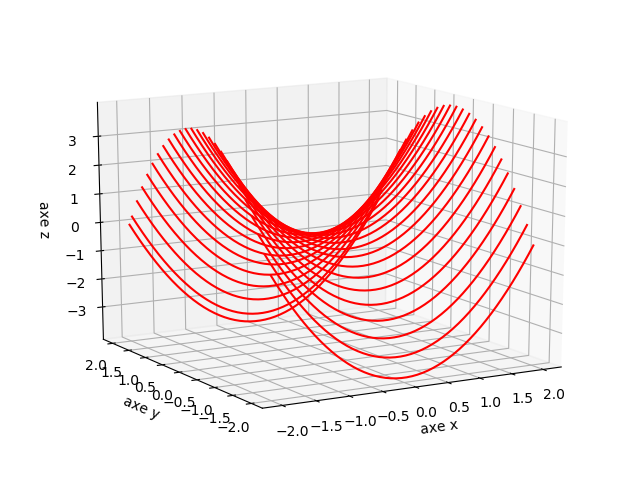
\includegraphics[scale=\myscale,scale=0.5]{figures/fonctions-quadra-3c}
    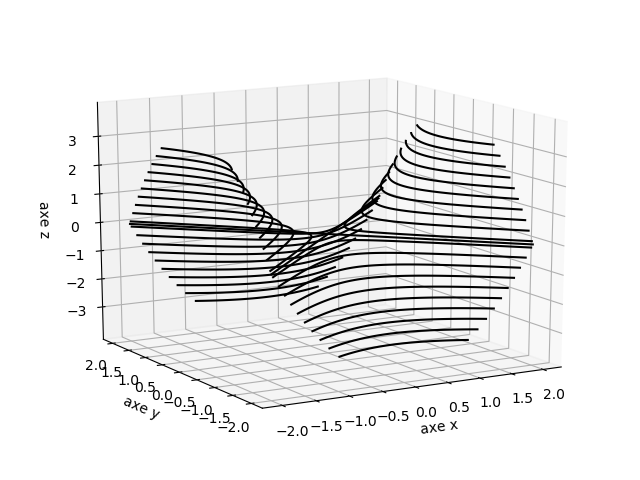
\includegraphics[scale=\myscale,scale=0.5]{figures/fonctions-quadra-3d}
    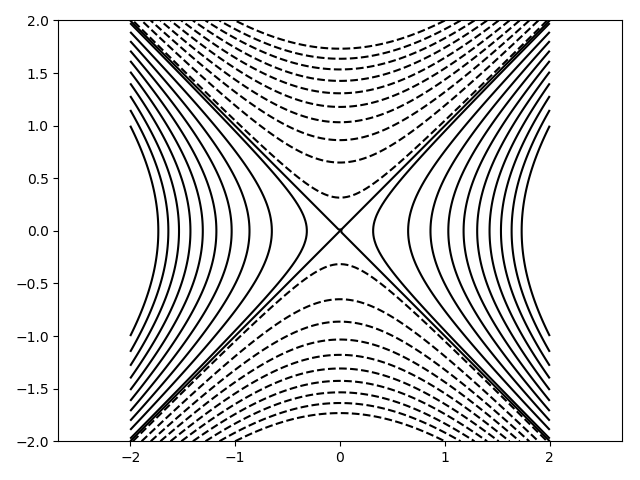
\includegraphics[scale=\myscale,scale=0.5]{figures/fonctions-quadra-3e}
\end{center}

% dessins 3d voir 'fonctions-quadra-3.py'

\end{exemple}



 
%----------------------------------------------------
\begin{miniexercices}
\sauteligne
\begin{enumerate}
  \item Déterminer et dessiner le domaine de définition de la fonction définie par $f(x,y) = \ln(xy)$.
  Même question avec $g(x,y) = \sqrt{2x-y^2+1}$ et $h(x,y,z) = \frac1x + \frac1y + \frac1z$.
   
  \item Déterminer l'image des fonctions de la question précédente.
  
  \item Soit $f(x,y) = xy$. Dessiner le graphe de $f$, les tranches et les lignes de niveau. Quelle surface reconnaissez-vous ? Vous pouvez vous aider d'un ordinateur. Mêmes questions avec $g(x,y) = -x^2-y^2$. 
  
\end{enumerate}
\end{miniexercices}


%%%%%%%%%%%%%%%%%%%%%%%%%%%%%%%%%%%%%%%%%%%%%%%%%%%%%
\section{Limites}


Les notions de limite et de continuité des fonctions d'une seule variable se généralisent en plusieurs variables sans complexité supplémentaire : il suffit de remplacer la valeur absolue par la norme euclidienne.


%----------------------------------------------------
\subsection{Définition}



Soit $f$ une fonction $f: E \subset \Rr^n \to \R$ définie au voisinage de $x_0 \in \Rr^n$, sauf peut-être en $x_0$.

\begin{definition}
La fonction $f$ admet pour \defi{limite} le nombre réel $\ell$ lorsque $x$ tend vers $x_0$ si : 
$$\forall \epsilon >0 \quad \exists \delta > 0 \qquad
\forall x\in E  \qquad 
0< \| x-x_0 \| <\delta \implies | f(x)-\ell | < \epsilon
$$
On écrit alors 
$$\lim_{x_0} f = \ell \qquad \text{ ou }\qquad \lim_{x \to x_0} f(x) = \ell \qquad \text{ ou } \qquad f(x) \underset{x\to x_0}{\longrightarrow} \ell.$$
\end{definition}

On définirait de même $\lim_{x \to x_0} f(x) = +\infty$ par :
$$\forall A >0 \quad \exists \delta > 0 \qquad
\forall x\in E  \qquad 
0< \| x-x_0 \| <\delta \implies | f(x) | > A
$$

\begin{remarque*}
\sauteligne
\begin{itemize}
\item La notion de limite ne dépend pas ici des normes utilisées.
\item Si elle existe, la limite est unique.
\end{itemize}
\end{remarque*}


\begin{exemple}
\label{ex:plusvarex}
Soit $f$ la fonction définie par $f(x,y) = x^2+y\sin(x+y^2)$.
\begin{enumerate}
  \item Montrer que $f(x,y)$ tend vers $0$ lorsque $(x,y) \to (0,0)$. 
  \item Trouver un ouvert $U$ contenant l'origine tel que, pour tout $(x,y) \in U$, on ait $| f(x,y) | < \frac{1}{100}$.
\end{enumerate}
  
\begin{center}
  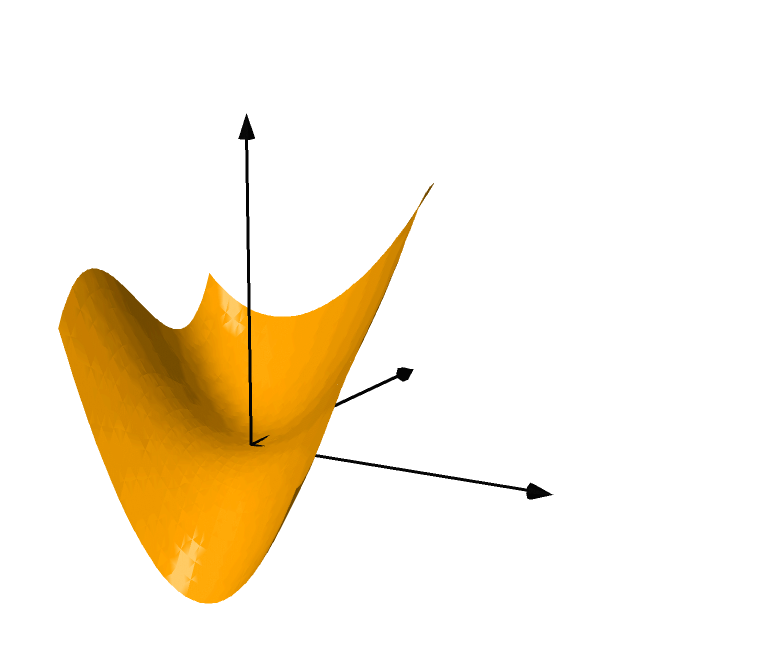
\includegraphics[scale=0.4]{figures/fig-plusvar-31-01}
\end{center}
 

\bigskip
\emph{Solution.}

\begin{enumerate}
  \item On majore $|f(x,y)|$ en utilisant l'inégalité triangulaire et $|\sin(t)| \le 1$ :
  $$\big| f(x,y) \big|  = \big| x^2+y\sin(x+y^2) \big| \le
  x^2 + |y| \big| \sin(x+y^2) \big| \le x^2 +|y|$$ 
  
  Fixons $0<\epsilon<1$. Fixons $a = \sqrt{\frac{\epsilon}{2}}$ et $b=\frac\epsilon2$. Alors, pour $x \in {}]-a,a[$, on a $x^2 < \frac\epsilon2$ et, pour $y \in {}]-b,b[$, on a $|y| < \frac\epsilon2$. Pour $(x,y) \in {}]-a,a[ \times  {}]-b,b[$, on a donc 
  $$\big| f(x,y) \big| \le x^2 +|y| < \frac\epsilon2 + \frac\epsilon2 = \epsilon.$$
  
  Une valeur $\delta$ qui convient est donc $\delta = \frac\epsilon2$. En effet,
  si $\| (x,y) \| < \delta$ alors $|x| < \delta = \frac\epsilon2 \le  \sqrt{\frac{\epsilon}{2}} $ 
  et $|y| < \delta = \frac\epsilon2$ donc $|f(x,y)| < \epsilon$. Conclusion : $f$ admet pour limite $0$ lorsque $(x,y)$ tend vers $(0,0)$.
  
\myfigure{1}{
  \tikzinput{fig-plusvar-31-02}
} 
  
  
  \item Pour $\epsilon = \frac{1}{100}$, on a $a = \frac{1}{\sqrt{200}}$ et $b=\frac{1}{200}$. Pour chaque $(x,y)$ de l'ouvert $]-a,a[ \times {}]-b,b[$, on a $|f(x,y)| < \frac{1}{100}$.
\end{enumerate}
  
\end{exemple}

%----------------------------------------------------
\subsection{Opérations sur les limites}


Pour calculer les limites, on ne recourt que rarement à cette définition. 
On utilise plutôt les théorèmes généraux : opérations sur les limites et encadrement. 
Ce sont les mêmes énoncés que pour les fonctions d'une variable : il n'y a aucune difficulté ni nouveauté. 


\begin{proposition}[Opérations sur les limites]
Soient $f,g:\Rr^n\to \Rr$ définies au voisinage de $x_0 \in \Rr^n$ et telles que $f$ et $g$ admettent des limites en $x_0$. Alors :
$$\lim_{x_0}(f+g)=\lim _{x_0}f+\lim _{x_0}g 
\qquad  \qquad 
\lim _{x_0}(f \cdot g)=\lim _{x_0}f\times \lim _{x_0}g$$
Et si $g$ ne s'annule pas dans un voisinage de $x_0$ :
$$\lim _{x_0}\frac{1}{g}=\frac{1}{\lim _{x_0}g} 
\qquad  \qquad 
\displaystyle \lim _{x_0}\frac{f}{g}=\frac{\lim _{x_0}f}{\lim _{x_0}g}
$$
\end{proposition}

\begin{remarque*}
\sauteligne
\begin{itemize}
  \item 
Les résultats ci-dessus sont aussi valables pour des limites infinies avec les conventions usuelles :
$$\ell+\infty =+\infty,\quad \ell-\infty =-\infty,\quad \frac{1}{0^+}=+\infty ,\quad \frac{1}{0^-}=-\infty ,\quad \frac{1}{\pm \infty }=0,$$
$$\ell\times \infty =\infty \; (\ell\neq 0),\; \infty \times \infty =\infty \text{ (avec règle de multiplication des signes).}$$

  \item 
Les formes indéterminées sont : $+\infty -\infty$, $\dfrac{0}{0}$, 
$\dfrac{\infty }{\infty}$, $0\times \infty$, , $\infty^0$, $1^{\infty}$ et $0^0$.
\end{itemize}
\end{remarque*}


La composition est aussi souvent utile : 
\begin{itemize}
  \item soit $f : \Rr^n \to \Rr$ une fonction de plusieurs variables, telle que $\lim_{x \to x_0} f(x) = \ell$,
  \item soit $g : \Rr \to \Rr$ une fonction d'une seule variable, telle que 
$\lim_{t \to \ell} g(t) = \ell'$,
  \item alors la fonction de plusieurs variables $g \circ f : \Rr^n \to \Rr$ définie par $(g \circ f) (x) = g \big( f(x) \big)$ vérifie
  $\lim_{x \to x_0} (g \circ f)(x) = \ell'$.
\end{itemize}

Application : grâce à l'exemple \ref{ex:plusvarex}, et comme $e^t \to 1$ lorsque $t\to 0$, on en déduit :
$$e^{x^2+y\sin(x+y^2)} \xrightarrow[(x,y) \to (0,0)]{} 1$$


\bigskip

Il existe aussi un théorème \og{}des gendarmes\fg{}.
\begin{theoreme}[Théorème d'encadrement] 
Soient $f,g,h:\Rr^n\to \Rr$ trois fonctions définies dans un voisinage $U$ de $x_0 \in \Rr^n$.
\begin{itemize}
  \item Si, pour tout $x \in U$, on a $f(x) \le  h(x) \le g(x)$,
  \item et si $\lim_{x_0} f = \lim_{x_0} g = \ell$,
\end{itemize}
alors $h$ admet une limite au point $x_0$ et $\displaystyle \lim _{x_0} h=\ell$.
\end{theoreme}



\begin{exemple}
Soit $h$ définie par $h(x,y) = \cos(x+y^2)\big( x^2+y\sin(x+y^2) \big)$.
On majore la valeur absolue du cosinus par $1$ :
$$\big| h(x,y) \big| \le \big|x^2+y\sin(x+y^2)\big| .$$
On a vu lors de l'exemple \ref{ex:plusvarex} que la fonction définie par
$f(x,y) = x^2+y\sin(x+y^2)$ tend vers $0$ en $(0,0)$. 
Donc, par le théorème des gendarmes, $h(x,y)$ tend aussi vers $0$ lorsque $(x,y)$ tend vers $(0,0)$.
\end{exemple}



%----------------------------------------------------
\subsection{Limite le long d'un chemin}

L'unicité de la limite implique que, quelle que soit la façon dont on arrive au point $x_0$, la valeur limite est toujours la même.

\begin{proposition} Soit $f:\Rr^n\to \Rr$ une fonction définie au voisinage de $x_0 \in \Rr^n$, sauf peut-être en $x_0$.
\begin{enumerate}
\item Si $f$ admet une limite $\ell$ au point $x_0$, alors la restriction de $f$ à toute courbe passant par $x_0$ admet une limite en $x_0$ et cette limite est $\ell$. 
\item Par contraposée, si les restrictions de $f$ à deux courbes passant par $x_0$ ont des limites différentes au point $x_0$, alors $f$ n'admet pas de limite au point $x_0$.
\end{enumerate}
\end{proposition}

Détaillons dans les cas des fonctions de deux variables :
\begin{itemize}
  \item Une courbe passant par le point $(x_0,y_0) \in \Rr^2$ est une fonction continue 
$\gamma : \Rr \to \Rr^2$, $t \mapsto (x(t),y(t))$, telle que $\gamma(0) = (x_0,y_0)$.
  \item La restriction de $f$ le long de $\gamma$ est la fonction d'une variable $f \circ \gamma$ : $t \mapsto f \big( x(t),y(t) \big)$.
  \item Si $f$ a pour limite $\ell$ en $(x_0,y_0)$ alors la première partie de la proposition affirme que 
  $f \big( x(t),y(t) \big) \underset{t \to 0}{\longrightarrow} \ell$.
\end{itemize}

\myfigure{1}{
  \tikzinput{fig-plusvar-33-01}
}

\begin{exemple}
Soit $f : \Rr^2 \to \Rr$ définie par 
$$f(x,y) = \frac{xy}{x^2+y^2} \text{ si } (x,y) \neq (0,0) \quad \text{ et } \quad
f(0,0) =0.$$

La fonction $f$ admet-elle une limite en $(0,0)$ ?

\bigskip
\emph{Solution.}

\begin{itemize}
  \item Si on prend le chemin $\gamma_1(t) = (t,0)$, alors 
  $(f \circ \gamma_1) (t) = f(t,0) = 0$. Donc, lorsque $t \to 0$, $(f \circ \gamma_1) (t) \to 0$.
  
  \item Si on prend le chemin $\gamma_2(t) = (t,t)$, alors 
  $(f \circ \gamma_2) (t) = f(t,t) = \frac{t^2}{2t^2} = \frac12$. Donc, lorsque $t \to 0$, $(f \circ \gamma_2) (t) \to \frac 12$.


Ci-dessous, sur la figure de gauche, les deux chemins du plan ; 
sur les deux figures de droite, deux vues différentes des valeurs prises par $f$ le long de ces chemins.

\begin{minipage}{0.25\textwidth}
\myfigure{0.6}{
  \tikzinput{fig-plusvar-33-02}
}
\end{minipage}
\begin{minipage}{0.79\textwidth}
\begin{center}
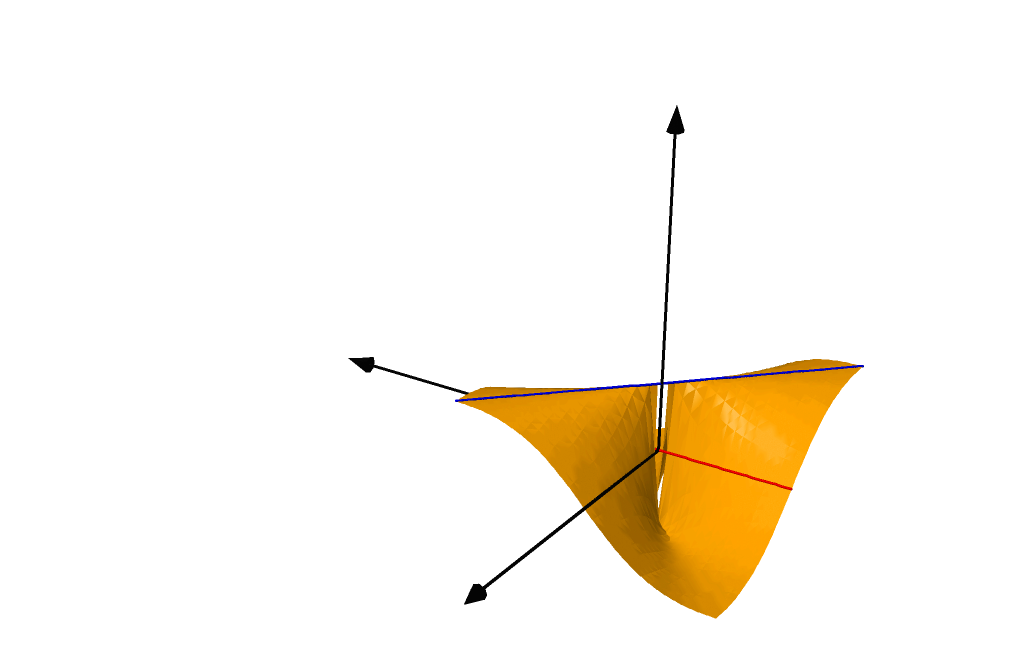
\includegraphics[scale=0.20]{figures/fig-plusvar-33-03a} 
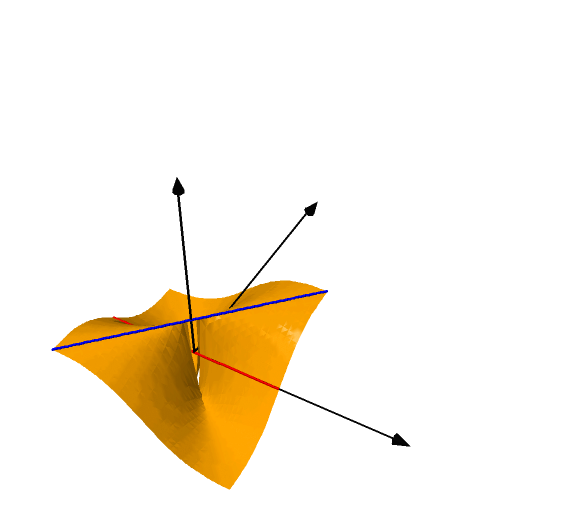
\includegraphics[scale=0.27]{figures/fig-plusvar-33-03b}  
\end{center}
\end{minipage}


   
  \item Si $f$ admettait une limite $\ell$ alors, quel que soit le chemin $\gamma(t)$ tel que $\gamma(t) \to (0,0)$ lorsque $t\to0$, on aurait  $(f \circ \gamma) (t) \to \ell$. 
  On aurait donc $\ell=0$ et $\ell=\frac12$, ce qui contredirait l'unicité de la limite. Ainsi, $f$ n'a pas de limite en $(0,0)$.
\end{itemize}
\end{exemple}

\bigskip
\bigskip

Une autre formulation possible : 

Si $f : \Rr^n\to \Rr$ a pour limite $\ell$ en $x_0 \in \Rr^n$ alors,
pour toute suite $(u_n)$ d'éléments de $\Rr^n$ telle que $u_n \to x_0$, on a $f(u_n) \to \ell$. 
Pour les fonctions de deux variables, cela s'écrit ainsi :
si $f$ a pour limite $\ell$ en $(a,b)$ alors, pour toute suite
$(a_n,b_n) \to (a,b)$, on a $f(a_n,b_n) \to \ell$.


%----------------------------------------------------
\subsection{Fonctions continues}


\begin{definition}
\sauteligne
\begin{enumerate}
\item $f : E \subset \Rr^n \rightarrow \Rr$ est \defi{continue en $x_0$} $\in E$ si $\displaystyle \lim_{x \rightarrow x_0} f(x) = f(x_0)$.
\item $f$ est \defi{continue sur $E$} si elle est continue en tout point de $E$.
\end{enumerate}
\end{definition}

Par les propriétés des limites, si $f$ et $g$ sont deux fonctions continues en $x_0$, alors : 
\begin{itemize}
\item la fonction $f + g$ est continue en $x_0$,
\item de même $fg$ et $f/g$ (avec $g(x) \neq 0$ sur un voisinage de $x_0$)  sont continues en $x_0$,
\item si $h : \Rr \to \Rr$ est continue, alors $h \circ f$ est continue en $x_0$.
\end{itemize}

\begin{exemple}
\sauteligne
\begin{itemize}
  \item Les applications définies par $(x,y)\mapsto x+y$, $(x,y)\mapsto xy$, puis 
  toutes les fonctions polynômes en deux variables $x$ et $y$ sont continues sur $\Rr^2$ (par exemple $(x,y)\mapsto x^2+3xy$). De la même façon, toutes les fractions rationnelles 
  en deux variables sont continues là où elles sont définies.
  
  \item Comme l'exponentielle est une fonction continue, alors $(x,y)\mapsto e^{xy}$ est continue sur $\Rr^2$.
  
  \item La fonction définie par $f(x,y) = \frac{1}{\sqrt{x^2 + y^2}}$ est continue sur $\Rr^2\setminus\{(0,0)\}$.
\end{itemize}
\end{exemple}
  


\begin{definition}[Prolongement par continuité]
Soit $f: E \subset \Rr^n \to \Rr$. Soit $x_0$ un point adhérent à $E$ 
n'appartenant pas à $E$. Si $f(x)$ a une limite $\ell$ lorsque $x \to x_0$,
on peut étendre le domaine de définition de $f$ à $E \cup \lbrace x_0 \rbrace$ en posant $f(x_0)=\ell$. 
La fonction étendue est continue en $x_0$. On dit que l'on a obtenu un \defi{prolongement de $f$ par continuité} au point $x_0$.
\end{definition}


\begin{exemple}
Soit $f : \Rr^2 \setminus \{ (0,0) \}$ définie par 
$$f(x,y) = \frac{xy}{\sqrt{x^2+y^2}}.$$

Est-il possible de prolonger $f$ par continuité en $(0,0)$ ?

Sur la figure ci-dessous, la question devient simplement : est-il possible de 
boucher le trou au milieu de la surface en rajoutant juste un point ?
\begin{center}
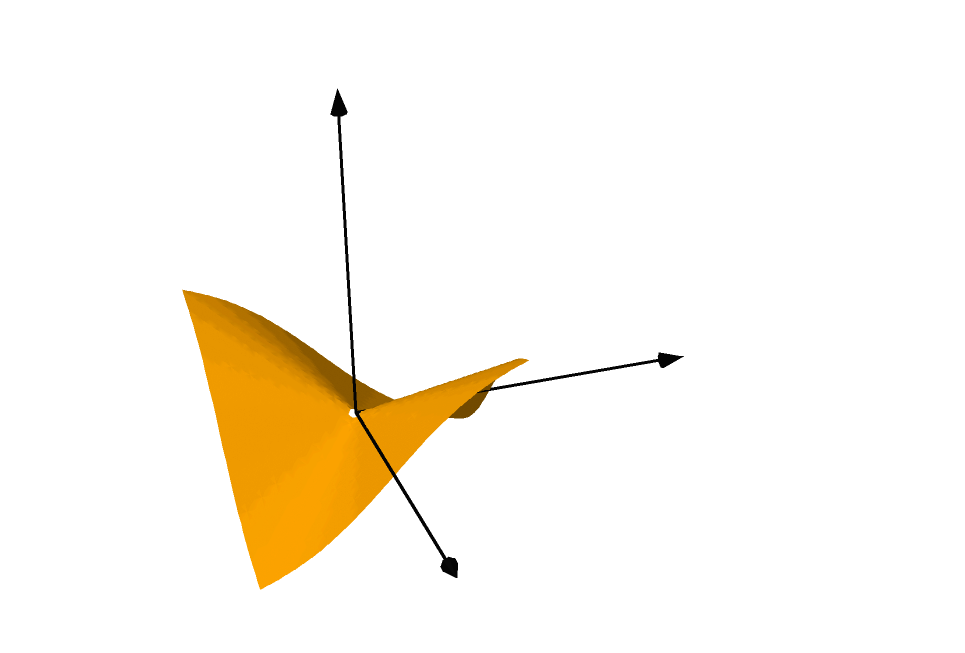
\includegraphics[scale=0.3]{figures/fig-plusvar-34-01}  
\end{center}

\bigskip
\emph{Solution.}

\begin{itemize}
  \item \textbf{Limite à l'origine.}
  
  On utilise que $|x| \le \sqrt{x^2+y^2}$ et $|y| \le \sqrt{x^2+y^2}$.
  Donc
  $$| f(x,y) |  = \frac{|x| \cdot |y|}{\sqrt{x^2+y^2}}
  \le \sqrt{x^2+y^2} \xrightarrow[(x,y) \to (0,0)]{} 0.$$
  
  \item \textbf{Prolongement.}
  
  Pour prolonger $f$ en $(0,0)$, on choisit comme valeur la limite obtenue.  
  On pose donc $f(0,0) = 0$. (On note encore $f : \Rr^2 \to \Rr$ la fonction prolongée.) 
  
  \item \textbf{Continuité.}
  
  Par notre choix de $f(0,0)$, $f$ est continue en $(0,0)$.
  En dehors de l'origine, $f$ est continue comme somme, produit, composition, inverse de fonctions continues. 
  Conclusion : la fonction prolongée est continue sur $\Rr^2$ tout entier.
\end{itemize}  
\end{exemple}


%----------------------------------------------------
\begin{miniexercices}
\sauteligne
\begin{enumerate}
  \item Soit $f(x,y) = \frac{1+x}{1+y}$. Trouver un ouvert $U$ contenant l'origine tel que 
  $0.999 < f(x,y) < 1.001$ pour tout $(x,y) \in U$.

  \item Soit $f : \Rr^n \rightarrow \Rr$ une fonction continue au point $(x_1,\ldots,x_n)$.
  Montrer que la fonction partielle $f_i : \Rr \longrightarrow \Rr$ définie par 
  $f_i(t) = f(x_1,\ldots,x_{i-1},t,x_{i+1},\ldots,x_n)$ est continue en $x_i$.
  
  \item Sachant que la limite de $f(x,y) = \frac{1+x}{1+y}$ en $(0,0)$ est $1$, calculer la limite des fonctions suivantes en $(0,0)$ : $\frac{1+x}{1+y}+ x^2+y^2$ ; $\frac{1+y}{1+x}$ ;   $\sin(xy)\frac{1+x}{1+y}$ ; $\ln\left(\frac{1+x}{1+y}\right)$.
  
  \item Sachant que $\ln(t) \le t-1$ pour tout $t>0$, calculer la limite de $\frac{\ln(1+xy)}{1+x^2+y^4}$ en $(0,0)$. 
  
  \item Soit $f(x,y)= \frac{\sin(x^2-y^2)}{x^2+y^2}$. Soit $\gamma(t) = (at,bt)$ où $(a,b) \in \Rr^2\setminus \{(0,0)\}$ est fixé. Calculer la limite de $(f \circ \gamma)(t)$ lorsque $t\to0$ en fonction de $(a,b)$. $f$ admet-elle une limite en $(0,0)$ ?  $f$ est-elle prolongeable par continuité en $(0,0)$ ? 
  
  
  \item Soit $f$ définie sur $\Rr^2\setminus \{ (0,0) \}$ par 
  $f(x,y) = \frac{xy^3}{x^2+2y^2}$. 
  $f$ admet-elle une limite en $(0,0)$ ? 
  $f$ est-elle prolongeable par continuité en $(0,0)$ ? 
  Mêmes questions avec $f(x,y)=\frac{xy^3}{x^4+2y^4}$.
  
\end{enumerate}
\end{miniexercices}



%%%%%%%%%%%%%%%%%%%%%%%%%%%%%%%%%%%%%%%%%%%%%%%%%%%%%
\section{Coordonnées polaires}


Plutôt que de repérer un point du plan $\Rr^2$ par ses coordonnées cartésiennes $(x,y)$, 
on peut le faire au moyen de sa distance à l'origine et de l'angle formé avec l'horizontale : ce sont les coordonnées polaires.


%----------------------------------------------------
\subsection{Définition}

Soit $M$ un point du plan $\Rr^2$. Soit $O=(0,0)$ l'origine. Soit $(O, \vec i, \vec j)$ un repère orthonormé direct.

\begin{itemize}
  \item On note $r = \| \overrightarrow{OM} \|$, la distance de $M$ à l'origine.
  \item On note $\theta$ l'angle entre $\vec i$ et $\overrightarrow{OM}$.
\end{itemize}

\myfigure{1}{
  \tikzinput{fig-plusvar-41-01}
}

On note $[r:\theta]$ les \defi{coordonnées polaires} du point $M$. Dans ce cours, $r$ sera toujours positif.
L'angle n'est pas déterminé de manière unique, plusieurs choix sont possibles. 
Pour avoir unicité, on peut limiter $\theta$ à l'intervalle $[0,2\pi[$, ou bien 
$]-\pi,+\pi]$. On n'attribue généralement pas de coordonnées polaires au point origine (l'angle n'aurait pas de sens). 

\bigskip
\evidence{Coordonnées polaires vers coordonnées cartésiennes.}

On retrouve les coordonnées cartésiennes $(x,y)$ à partir des coordonnées polaires $[r:\theta]$ par les formules
$$x = r\cos \theta \qquad\text{ et }\qquad y = r \sin \theta.$$

Autrement dit, on a défini une application :
$$
]0,+\infty[\times[0,2\pi[\rightarrow \Rr^2 \qquad (r,\theta)\mapsto (r\cos\theta,r\sin\theta).
$$

\bigskip
\evidence{Coordonnées cartésiennes vers coordonnées polaires.}

On retrouve  $r$ et $\theta$ à partir de $(x,y)$ par les formules suivantes :
$$r = \sqrt{x^2+y^2}$$
et, dans le cas $x>0$ et $y\ge0$, 
$$\theta = \arctan\left(\frac yx\right).$$

Pour les points dans les autres quadrants, on se ramène au quadrant principal où $x>0$ et $y\ge0$.



%----------------------------------------------------
\subsection{Limite et continuité}


Lorsque l'on considère des applications $f: E \subset \Rr^2 \rightarrow \R$, il est quelquefois plus facile de prouver des résultats de limite, continuité, etc., en passant par les coordonnées polaires.


\begin{proposition}
\label{prop:limrtheta}
Soit $f:\Rr^2\to \Rr$ une fonction définie au voisinage de $(0,0)\in \Rr^2$, sauf peut-être en $(0,0)$. Si
$$\lim _{r\to 0}f(r\cos \theta ,r\sin \theta )=\ell \in \Rr$$
existe indépendamment de $\theta$, c'est-à-dire
qu'il existe une fonction $\epsilon(r)\underset{r\to0}{\longrightarrow}0$ telle que, pour tout $r\ge0$ et tout $\theta$, on a :
$$\big| f(r\cos \theta ,r\sin \theta ) - \ell \big| \le \epsilon(r),$$
alors $\displaystyle \lim _{(x,y)\to (0,0)}f(x,y)=\ell$.
\end{proposition}


Pour clarifier cette proposition et expliquer les différents cas pratiques de la limite, voici comment faire. On exprime $f(x,y)$ en coordonnées polaires en calculant $f(r\cos\theta,r\sin\theta)$.
\begin{enumerate}
  \item Si $\lim_{r\to0} f(r\cos\theta,r\sin\theta)$ existe et si elle ne dépend pas de la variable $\theta$, alors cette limite est la limite de $f$ au point $(0,0)$.
  
  \item Si $\lim_{r\to0} f(r\cos\theta,r\sin\theta)$ n'existe pas, alors $f$ n'a pas de limite au  point $(0,0)$.
  
  \item Si $\lim_{r\to0} f(r\cos\theta,r\sin\theta) = \ell(\theta)$ dépend de $\theta$, alors $f$ n'a pas de limite au  point $(0,0)$. Pour le justifier, on donne deux valeurs $\theta_1$ et $\theta_2$ telles que $\ell(\theta_1) \neq \ell(\theta_2)$.
  
\end{enumerate}


Voyons un exemple de chaque situation.

\begin{exemple}
\sauteligne
\begin{enumerate}
  \item $f(x,y)=\dfrac{x^3}{x^2+y^2}$
  
  $$f(r\cos\theta,r\sin\theta) = \frac{r^3 \cos^3\theta}{r^2 (\cos^2\theta+\sin^2\theta)}
  = \frac{r^3 \cos^3\theta}{r^2} = r \cos^3 \theta$$
  Comme $\big| \cos^3 \theta \big| \le 1$ alors $r |\cos^3 \theta| \le r$ (pour tout $r$ mais aussi pour tout $\theta$) avec $\epsilon(r) := r \underset{r\to0}{\longrightarrow} 0$.  
  Ce qui implique que $f(r\cos\theta,r\sin\theta) \underset{r\to0}{\longrightarrow} 0$.
  La limite existe (indépendamment des valeurs prises par $\theta$), donc 
  la fonction $f$ admet bien une limite en $(0,0)$ : $f(x,y) \xrightarrow[(x,y) \to (0,0)]{} 0$.
  
  Pour ceux qui voudraient tout faire à la main avec plus de détails, on peut aussi écrire $\big|f(r\cos\theta,r\sin\theta)\big| \le r$, autrement dit $\big|f( x,y) \big| \le \sqrt{x^2+y^2}$. Donc $f(x,y) \xrightarrow[(x,y) \to (0,0)]{} 0$.
  
   
  \item $f(x,y)=\dfrac{y}{x^2+y^3}$
  
  
 $$f(r\cos\theta,r\sin\theta) = \frac{r\sin\theta}{r^2(\cos^2\theta + r\sin^3\theta)} = \frac{1}{r} \frac{\sin\theta}{\cos^2\theta + r\sin^3\theta}$$
 
Fixons $\theta$ tel que $\sin \theta \neq 0$ (c'est-à-dire $\theta \neq 0 \pmod \pi$). Alors, lorsque $r\to0$, $f(r\cos\theta,r\sin\theta)$ n'a pas de limite. En particulier, la fonction $(x,y) \mapsto f(x,y)$ n'a pas de limite en $(0,0)$.
 
  
  \item  $f(x,y)=\dfrac{xy}{x^2+y^2}$
  
 $$f(r\cos\theta,r\sin\theta) = \frac{r^2 \cos\theta\sin\theta}{r^2}
  = \cos\theta \sin \theta = \frac12\sin(2\theta)$$ 

Pour $\theta$ fixé, la fonction $r \mapsto f(r\cos\theta,r\sin\theta)$ admet bien une limite $\ell(\theta) = \frac12\sin(2\theta)$, lorsque $r\to0$. Mais cette limite dépend de l'angle $\theta$ :
si $\theta =0$, $\ell(\theta)=0$ ; par contre, si $\theta = \frac\pi4$, $\ell(\theta) = \frac12$. Comme la limite dépend de l'angle, alors la fonction de deux variables $(x,y) \mapsto f(x,y)$ n'a pas de limite en $(0,0)$.
\end{enumerate}
\end{exemple}

 

%----------------------------------------------------
\subsection{Un exemple}

Cet exemple est assez subtil et peut être passé en première lecture.

\begin{remarque*}
Soit $\ell \in \Rr$. Soit $f: \Rr^2 \rightarrow \Rr$ une fonction telle que, pour chaque $\theta$ fixé, $\displaystyle \lim_{r \to0} f(r\cos\theta, r\sin\theta)=\ell$. Peut-on en conclure que $f$ admet $\ell$ pour limite au point $(0,0)$ ? La réponse est non !

Autrement dit, regarder la limite de $f$ le long des rayons ne permet pas de trouver la limite de $f$ à l'origine.
\end{remarque*}

Attention : la différence entre cette remarque et la proposition \ref{prop:limrtheta} est subtile. Dans la proposition \ref{prop:limrtheta}, on a une hypothèse en terme de limites du type :
$$\forall \epsilon \quad \exists r_0 \quad \forall r<r_0 \quad \forall \theta \quad  \quad \cdots$$
alors que dans la remarque, on note que l'hypothèse (plus faible) suivante est insuffisante :
$$ \forall \theta \quad \forall \epsilon \quad \exists r_0 \quad \forall r<r_0 \quad \ldots$$


\begin{exemple}
Soit la fonction $f$ définie sur $\Rr^2 \setminus \{(0,0)\}$ par
$$f(x,y)=\frac{xy^2}{x^2+y^4}.$$
\begin{enumerate}
  \item Le long de tous les rayons $f$ tend vers $0$, c'est-à-dire, pour $\theta$ fixé,
$$f(r\cos\theta,r\sin\theta) \underset{r \to 0}{\longrightarrow} 0.$$
  \item Cependant, $f$ n'a pas de limite en $(0,0)$.
\end{enumerate}


\bigskip
\emph{Solution.}
\begin{enumerate}
  \item Calculons d'abord :
  $$f(r\cos\theta,r\sin\theta) 
  = \frac{r\cos\theta\sin^2\theta}{\cos^2\theta + r^2\sin^4\theta}$$
  
  Fixons $\theta$ et discutons selon sa valeur :
  \begin{itemize}
    \item Si $\cos\theta \neq 0$, alors le numérateur tend vers $0$, tandis que le dénominateur tend vers $\cos^2\theta \neq0$. Donc $f(r\cos\theta,r\sin\theta) \to 0$ lorsque $r\to0$.
    
    \item Si $\cos\theta = 0$, alors on se trouve sur des points $(x,y)$ où $x=0$ et donc 
    $f(r\cos\theta,r\sin\theta)=f(0,y)=0$.    
  \end{itemize}
  Dans tous les cas, $f$ tend vers $0$ sur tous les rayons définis par un angle $\theta$ fixé.
  
  
  \item Considérons le chemin $\gamma(t) = (t^2,t)$. Alors 
  $$(f \circ \gamma)(t) = \frac{t^4}{2t^4} = \frac12.$$
  Mais on a vu que le long des rayons $f$ tend vers $0$. 
  Cela contredit l'existence d'une limite pour $f(x,y)$ en $(0,0)$.
 
  \myfigure{1}{
  \tikzinput{fig-plusvar-43-01}
  }

\end{enumerate}  

\end{exemple}
 
%----------------------------------------------------
\begin{miniexercices}
\sauteligne
\begin{enumerate}

 \item Calculer l'angle $\theta$ des coordonnées polaires $[r:\theta]$ 
 d'un point $(x,y)$ dans le cas $x>0$, $y <0$. 
 Puis faire les cas où $x<0$.

  \item La fonction $f$ définie par $f(x,y)=\frac{(2x+3y)^3}{x^2+y^2}$  
  admet-elle une limite au point $(0,0)$ ?
  Même question avec $f(x,y)=\frac{(2x+3y)^2}{x^2+y^2}$, puis $f(x,y)=\frac{2x+3y}{x^2+y^2}$.

\end{enumerate}
\end{miniexercices}



\auteurs{
\\
Arnaud Bodin.
D'après des cours de Abdellah Hanani (Lille), 
Goulwen Fichou et Stéphane Leborgne (Rennes),
Laurent Pujo-Menjouet (Lyon). 
Relu par Anne Bauval, Vianney Combet et Barbara Tumpach.
}

\finchapitre 
\end{document}


